

\section{Need for \pulse}
\label{sec:needforpulse}


Disaggregated systems like \mind use small DRAM caches on CPU nodes while accessing memory across network-attached memory nodes with large DRAM pools (Fig.~\ref{fig:disagg}~(top)). However, limited bandwidth and latency of network-attached memory remain a challenge, constrained by the speed of light. Even with near-terabit links and RDMA~\cite{rdmalatency}, remote memory is much slower than local memory~\cite{disagg}. CXL interconnects~\cite{cxl} show similar patterns, with $300$ ns latency compared to $10$--$20$ ns for L3 cache~\cite{pond}. 

CPU caches can reduce average memory access latency, but their effectiveness is limited by data locality and cache size. Remote memory access is unavoidable for pointer-heavy applications, such as database index lookups~\cite{hash1, hash2, hash3, succinct, trie2, btree1, btree2, trie1, blowfish, trie3, surf} and graph analytics~\cite{powergraph, graphx, graphchi, pagerank} (Fig.~\ref{fig:motivation}). Memory-intensive applications~\cite{scuba, cachelib, tao, memcache, flighttracker, twittercache, spark} often require traversing linked structures like lists, hash tables, trees, and graphs. Despite large memory pools in disaggregated architectures, network pointer traversals remain slow~\cite{disagg}. Recent systems~\cite{disagg, legoos, mind, infiniswap, fastswap} mitigate this by caching hot data in CPU DRAM, but pointer traversals still suffer, as we demonstrate next.

\paragraphb{Pointer traversals in real-world workloads} Studies~\cite{graphchi, monetdb, spark, voltdb, memc3, db1000, memcached} show that cloud applications spend 21\% to 97\% of their execution time on pointer traversals. We analyzed three representative cloud applications — a WebService frontend~\cite{aifm}, WiredTiger indexing~\cite{wiredtiger}, and BTrDB time-series analysis~\cite{btrdb} — using swap-based disaggregated memory~\cite{infiniswap}. Varying the CPU cache size from $6.25\%$ to $100\%$ of the working set, Fig.~\ref{fig:motivation_experiment} shows that (i) significant execution time is spent on pointer traversals (13.6\%, 63.7\%, and 55.8\% respectively, even with full cache), and (ii) traversal time increases as CPU cache size decreases.

\paragraphb{Distributed traversals} As application workloads and working-set sizes grow, disaggregated systems allocate memory across multiple memory nodes~\cite{legoos, mind, infiniswap, fastswap}. To optimize load balancing and utilization, they use fine-grained allocations (e.g., $1$ GB in~\cite{legoos}, $2$ MB in~\cite{mind}), but this fragments linked structures across memory nodes, leading to frequent distributed traversals.

Fig.~\ref{fig:distributed_percentage} illustrates this for WiredTiger and BTrDB on a setup with $1$ compute and $4$ memory nodes: over 97\% and 75\% of requests, respectively, cross memory node boundaries. Fig.~\ref{fig:distributed_cdf_wiredtiger} shows the CDF of memory node crossings. While WiredTiger’s randomly ordered data requires frequent crossings, BTrDB’s time-ordered data confines larger allocations to the same node, reducing crossings. However, smaller allocations, necessary for high utilization, still result in many cross-node traversals.


\begin{figure}[t]
  \centering
  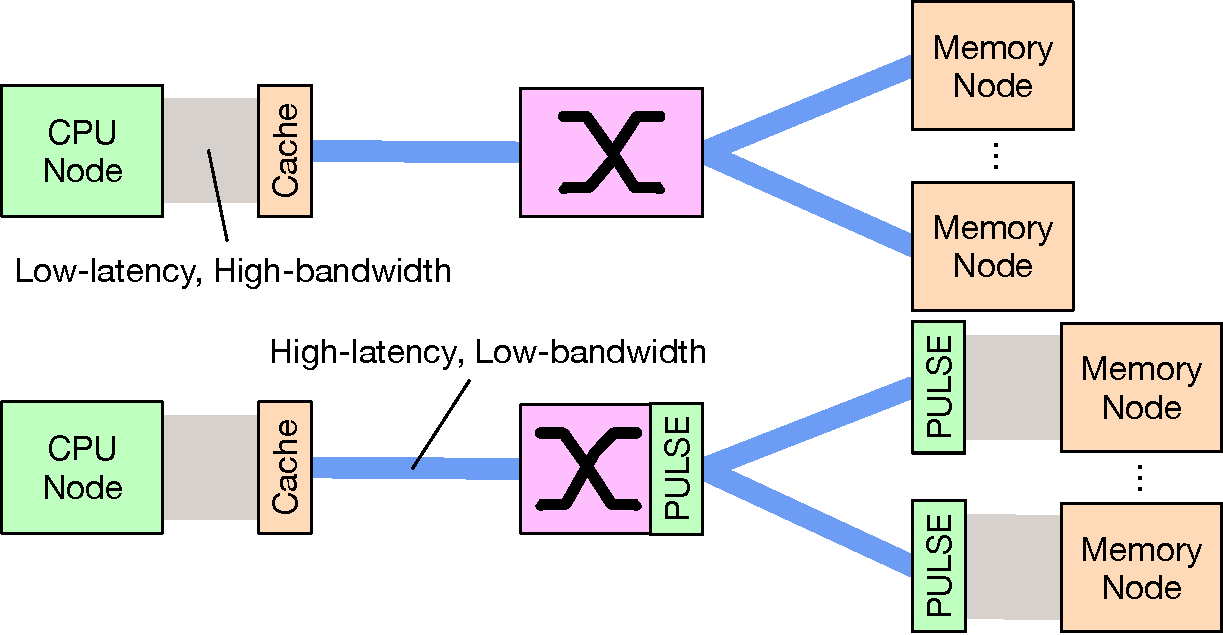
\includegraphics[width=0.6\textwidth]{fig/pulse/disagg_vertical.pdf}
  \caption[Need for accelerating pointer traversals]{\textbf{Need for accelerating pointer traversals.} \textit{(top)} Pointer traversals in disaggregated architectures are limited by slow memory interconnects. \textit{(bottom)} Like CPU caches, we propose a fast, lightweight accelerator for cache-unfriendly pointer traversals in traversal-heavy workloads.} 
  \label{fig:disagg}
\end{figure}

\begin{figure*}[ht!]
    \centering
    \subfigure[Our empirical analysis]{
        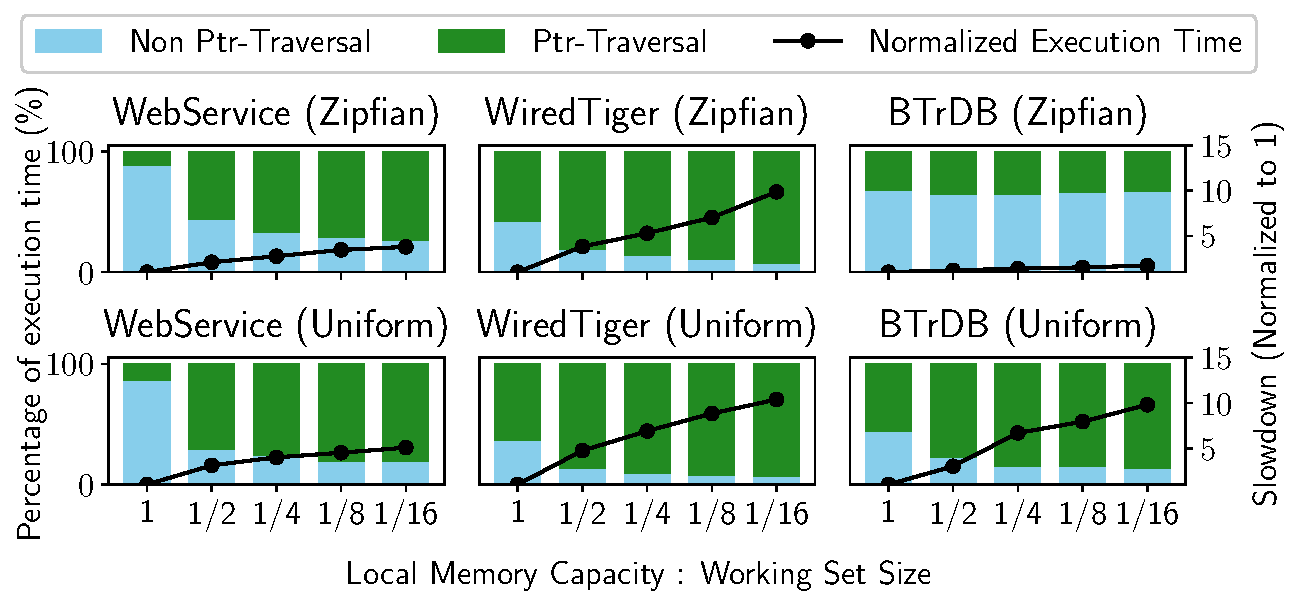
\includegraphics[width=0.43\textwidth]{fig/pulse/figure1_motivation.pdf}
        \label{fig:motivation_experiment}
    }
    \subfigure[\% of distributed traversals]{
        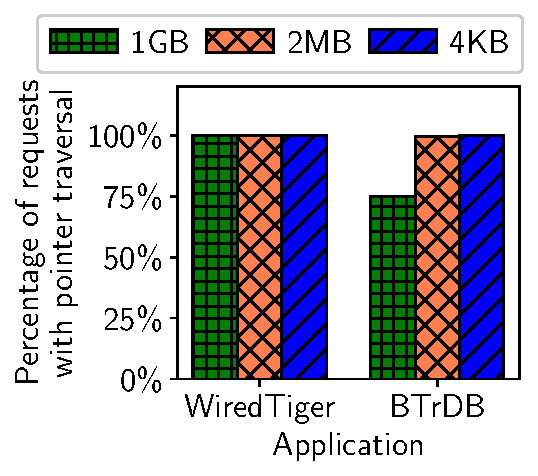
\includegraphics[width=0.23\textwidth]{fig/pulse/distributed.pdf}
        \label{fig:distributed_percentage}
    }
    \subfigure[CDF of distributed traversals]{
        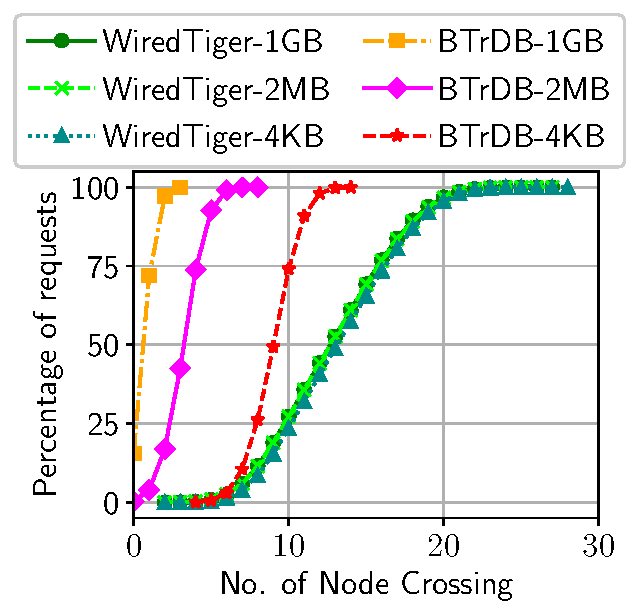
\includegraphics[width=0.27\textwidth]{fig/pulse/cdf.pdf}
        \label{fig:distributed_cdf_wiredtiger}
    }
    \caption[Time cloud applications spend in pointer traversals.]{\textbf{Time cloud applications spend in pointer traversals.}} 
    \label{fig:motivation}
\end{figure*}

Similar to the role of CPU caches in providing quick access to frequently used data, we propose augmenting memory nodes with lightweight, fast processing units that offer high-bandwidth, low-latency access for accelerating pointer traversals (Fig.~\ref{fig:disagg}~(bottom)). Additionally, the interconnect must enable efficient and scalable traversals across multiple memory nodes to handle large, linked data structures.

We introduce \pulse\footnote{\textbf{P}rocessing \textbf{U}nit for \textbf{L}inked \textbf{S}tructur\textbf{E}s.}, a distributed framework designed for efficient pointer traversals in rack-scale disaggregated memory systems. \pulse addresses three critical aspects—expressiveness, energy efficiency, and performance—by adopting a novel near-memory processing paradigm. At the heart of \pulse is an expressive iterator interface that provides a unified abstraction for pointer traversals in a variety of applications, including key-value stores~\cite{redis, memcached}, databases~\cite{wiredtiger, btree1, btree2, trie1, trie3}, and big-data analytics frameworks~\cite{powergraph, graphx, graphchi, pagerank} (\S\ref{ssec:pulseinterface}). This abstraction supports a wide range of traversal-heavy workloads, enabling (i) seamless integration with existing toolchains and (ii) the deployment of hardware accelerators optimized for iterators.

To ensure efficient pointer traversals, \pulse introduces a novel accelerator that decouples the logic and memory pipelines, leveraging the sequential nature of iterator execution (\S\ref{ssec:pulsearchitecture}). This design enables high memory utilization by balancing memory capacity with fewer logic pipelines. A scheduler distributes the traversal logic across multiple pipelines, employing multiplexing to maximize resource utilization. While our initial implementation of \pulse leverages FPGA-based SmartNICs due to the complexity of ASIC design, the framework is ultimately aimed at an ASIC-based implementation for higher efficiency.

For distributed traversals, \pulse employs a programmable network switch, treating pointer traversals across memory nodes similarly to packet routing (\S\ref{ssec:pulsedistributed}). The switch inspects iterator requests and routes them to the appropriate memory node at line rate. We have implemented a prototype using commodity servers, SmartNICs, and a programmable switch, making minimal hardware and software changes to ensure non-invasive deployment in existing infrastructures.






\begin{figure*}[ht!]
  \centering
  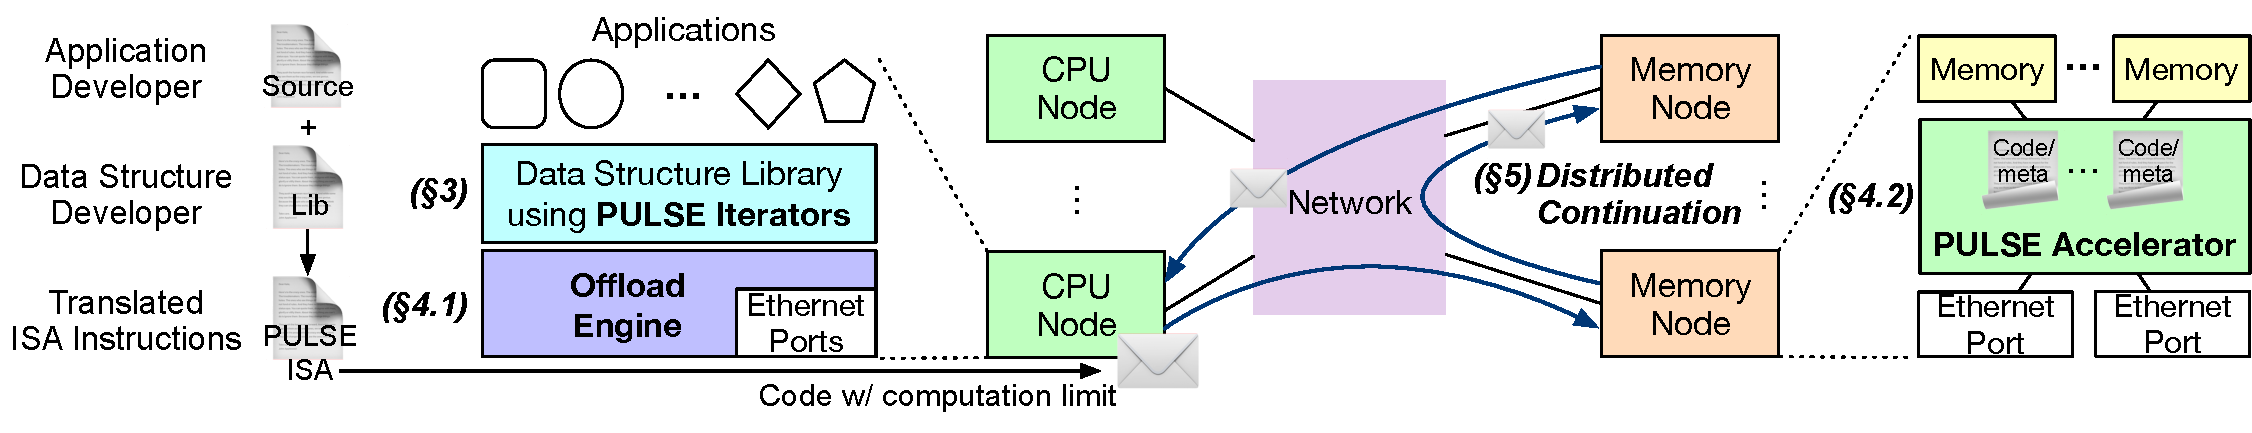
\includegraphics[width=\textwidth]{fig/pulse/overview.pdf}
  \caption[\pulse Overview]{\textbf{\pulse Overview.} Developers use \pulse's iterator interface (\S\ref{ssec:pulseinterface}) to express pointer traversals, translated to \pulse ISA by its dispatch engine (\S\ref{ssec:compute_node}). During execution, \pulse accelerator ensures energy efficiency (\S\ref{ssec:pulsearchitecture}) and in-network design enable distributed traversals (\S\ref{ssec:pulsedistributed}).} 
  \label{fig:general}
\end{figure*}


\section{\pulse Design}
\label{sec:pulsedesign}
\pulse introduces innovations across three key design elements (Fig.~\ref{fig:general}). At its core, \pulse's iterator-based programming model (\S\ref{ssec:pulseinterface}) simplifies the process of porting real-world data structure traversals. It supports \emph{stateful} traversals using a \emph{scratchpad}, which allows developers to store and update intermediate states (e.g., aggregators, arrays) during the execution of iterators. This iterator-based approach enables both tractable accelerator design and efficient distributed traversals.

The developer's iterator code is translated into \pulse's ISA (Instruction Set Architecture) for execution by \pulse accelerators (\S\ref{ssec:pulsearchitecture}). The accelerator achieves energy efficiency and high performance by decoupling logic and memory pipelines, with an ISA specifically tailored for the iterator pattern. A specialized scheduler is employed to maximize utilization and performance in this disaggregated architecture.

For scalable distributed pointer traversals, \pulse leverages programmable network switches to reroute requests that cross memory node boundaries (\S\ref{ssec:pulsedistributed}). Hierarchical address translation is performed \emph{in-network}, with the network switch managing memory node-level translation, while the accelerators at each memory node handle local address translation and memory protection. If a request cannot be handled locally, the accelerator returns it to the switch for rerouting to the appropriate memory node.

\paragraphb{Assumptions} \pulse relies on the CPU node for synchronization, requiring the application to explicitly handle locks. Although recent work enables locking mechanisms on NICs~\cite{sherman, clover} and switches~\cite{netlock}, these efforts are orthogonal and could be incorporated into \pulse. Additionally, \pulse adopts the caching scheme from prior work~\cite{aifm}, maintaining a transparent cache within the data structure library.



\subsection{\pulse Programming Model}
\label{ssec:pulseinterface}
We begin by discussing \pulse's programming model, as a well-designed interface is essential for supporting real-world traversal-heavy applications and for enabling the development of efficient pointer traversal accelerators and distributed mechanisms. \pulse's interface is specifically designed for data structure library developers, allowing them to offload pointer traversals within linked structures. Since the required code modifications are confined to the data structure libraries, applications that use these libraries can operate without any changes.

After analyzing various popular data structures~\cite{stl, boost, javaiterator, c++iterator}, we identified a common traversal pattern: (1) initializing a start pointer, (2) iteratively computing the next pointer, and (3) checking a termination condition at the end of each iteration. This pattern closely aligns with the \emph{iterator} design motif, which is widely adopted across different programming languages~\cite{javaiterator}. Consequently, \pulse adopts the iterator interface as the hardware-software boundary for handling pointer traversals (Listing~\ref{lst:iterator}).

The interface exposes three user-defined functions: (1) \code{init()} initializes the starting pointer based on the data structure, (2) \code{next()} updates the current pointer to the next element, and (3) \code{end()} checks whether the traversal should terminate. \pulse uses these functions to iteratively execute the traversal through \code{execute()}. Additionally, we introduce two key features in our iterator abstraction to both enhance and constrain the expressiveness of operations on linked data structures.


\begin{figure}[th]
\centering
\begin{lstlisting}[caption={\pulse interface.},label={lst:iterator},escapechar=|,basicstyle=\footnotesize,linewidth=\linewidth]
class pulse_iterator {
    void init(void *) = 0; // Implemented by developer
    void *next() = 0; // Implemented by developer
    bool end() = 0; // Implemented by developer
    
    unsigned char *execute() { // Non-modifiable logic
      unsigned int num_iter = 0;
      while (!end() && num_iter++ < MAX_ITER)
        cur_ptr = next();
      return scratch_pad;|\label{line:scratch_return}|
    }
    uintptr_t cur_ptr;
    unsigned char scratch_pad[MAX_SCRATCHPAD_SIZE];
}
\end{lstlisting}
\end{figure}

\begin{figure*}[th]
\centering
\begin{lstlisting}[caption={C++ STL realization for \code{unordered\_map::find()}.},label={lst:stl},escapechar=|,basicstyle=\footnotesize,linewidth=\linewidth]
struct node {
  key_type key;
  value_type value;
  struct node *next;
};

value_type find(key_type key) {
  for (struct node *cur_ptr = bucket_ptr(hash(key)); ; cur_ptr = cur_ptr->next) {
    if (key == cur_ptr->key) // Key found
      return cur_ptr->value;
    if (cur_ptr->next == nullptr) // Key not found
      break;
  }
  return KEY_NOT_FOUND;
}
\end{lstlisting}
\begin{lstlisting}[caption={\pulse realization for \code{unordered\_map::find()}.},label={lst:stl_mod},escapechar=|,basicstyle=\footnotesize,linewidth=\linewidth]
class unordered_map_find : pulse_iterator {
  init(void *key) {
    memcpy(scratch_pad, key, sizeof(key_type));
    cur_ptr = bucket_ptr(hash((key_type)*key));
  }
  
  void* next() { return cur_ptr->next; }
  
  bool end() {
    key_type key = *((key_type *)scratch_pad);
    if (key == cur_ptr->key) { // Key found
      *((value_type *)scratch_pad) = cur_ptr->value;
      return true;
    }
    if (cur_ptr->next == nullptr) { // Key not found
      *((unsigned int *)scratch_pad) = KEY_NOT_FOUND;  
      return true;
    }
    return false;
  }
}
\end{lstlisting}
\end{figure*}
  
  
  
\paragraphb{Stateful traversals} Pointer traversals in data structures are often stateful, with different types of state depending on the application. For example, in hash table lookups, the state is the search key, whereas in B-Tree summations, a running total is maintained and updated with each value. To support such operations, \pulse iterators include a \code{scratch\_pad} for storing arbitrary state. The state is initialized in \code{init()}, updated during each iteration in \code{next()}, and finalized in \code{end()}. Upon completion, the \code{execute()} function returns the contents of \code{scratch\_pad} (Line~\ref{line:scratch_return}), allowing developers to retrieve the result of the traversal.

\paragraphb{Bounded computations} \pulse accelerators facilitate lightweight processing for memory-intensive operations, ensuring efficient utilization of bandwidth. While \code{init()} is executed on the CPU, the \code{next()} and \code{end()} functions are offloaded to \pulse accelerators. These accelerators enforce two constraints on memory accesses and computations. First, \pulse disallows nondeterministic behavior, such as unbounded loops that cannot be unrolled. Second, \code{execute()} (as shown in Listing~\ref{lst:iterator}) limits the maximum number of iterations per request to prevent long-running traversals from monopolizing resources. If this limit is reached, \pulse terminates the traversal and returns the current \code{scratch\_pad} value to the CPU, allowing a new request to continue from the last point.

\paragraphb{An illustrative example} To demonstrate, we adapt the \code{find()} operation from the C++ STL \code{unordered\_map} to \pulse. Listing~\ref{lst:stl} shows a simplified STL implementation, where the traversal begins by computing a hash function to locate the corresponding hash bucket pointer, followed by iterating through the linked list in that bucket. The traversal ends when the key is found or when the list terminates.

In Listing~\ref{lst:stl_mod}, the \pulse iterator implementation is presented. The core logic remains largely unchanged, with modifications made to the \code{init()}, \code{next()}, and \code{end()} functions. The key differences involve how the state (the search key) is passed between these functions and how results (either an error message if the key is not found or its value if it is) are returned via the \code{scratch\_pad}.

\subsection{\pulse Dispatch Engine}
\label{ssec:compute_node}
The dispatch engine is a software framework running on the CPU node, designed for two key purposes. First, it translates the iterator-based pointer traversal code provided by data structure library developers (\S\ref{ssec:pulseinterface}) into \pulse's ISA. Second, it determines whether the accelerator can handle the computations required during the traversal, and if so, sends the request to the accelerator at the memory node. If the accelerator is unsuitable, execution proceeds on the CPU with regular remote memory accesses.

\paragraphb{Translating iterator code to \pulse ISA} To integrate seamlessly with existing workflows, \pulse plugs into standard compiler toolchains. The dispatch engine generates \pulse ISA instructions using well-established compiler techniques~\cite{llvm}. \pulse's ISA is a streamlined RISC instruction set, designed with only the essential operations for basic processing and memory access, optimizing for simplicity and energy efficiency (Table~\ref{tab:isa}). However, there are a few notable features in the adaptation of the iterator code to \pulse's ISA. 

First, as discussed in \S\ref{ssec:pulseinterface}, \pulse does not support unbounded loops within a single iteration. The ISA only supports conditional jumps that move forward in the code, akin to eBPF programs~\cite{ebpfjump}, which allow only forward jumps to prevent infinite execution within the kernel. A backward jump can occur only at the start of the next iteration; \pulse includes a specific \code{NEXT\_ITER} instruction to explicitly mark this point, enabling the accelerator to begin scheduling the memory pipeline (\S\ref{ssec:pulsearchitecture}). 

Second, developers can maintain state and return values using the \code{scratch\_pad}, which has a pre-configured size. \pulse's ISA supports direct register operations on the \code{scratch\_pad} and includes a \code{RETURN} instruction, which ends the iterator's execution and returns the contents of the \code{scratch\_pad} as the result.

Lastly, we observed that iterator traversal typically involves two main types of operations: fetching data\footnote{While this section focuses on data fetches, writing data to memory follows a similar process.} from memory via the \code{cur\_ptr} and processing that data to determine the next pointer or whether the traversal should terminate. If the translation of iterator code to \pulse's ISA is done naively, it may result in multiple redundant loads near the memory location pointed to by \code{cur\_ptr}. For example, in the \code{unordered\_map::find()} implementation in Listing~\ref{lst:stl_mod}, references to \code{cur\_ptr->key}, \code{cur\_ptr->value}, and \code{cur\_ptr->next} occur at different points, and each could incur a separate memory load, slowing down execution and wasting memory bandwidth. To address this, \pulse's dispatch engine uses static analysis to infer the range of memory locations accessed relative to \code{cur\_ptr} in the \code{next()} and \code{end()} functions and aggregates these accesses into a single large \code{LOAD} (up to 256 B) at the beginning of each iteration.


% \begin{figure*}
\begin{table}[btp!]
    \centering
    \footnotesize  % 8 pt for 10 pt body (small for 9pt)
    \def\arraystretch{0.98}%
    % \footnotesize % 8 pt for 10 pt body
    % \resizebox{0.475\textwidth}{!}{
    \begin{tabular}{l|l|l}
      \hline
      \textbf{Class}  & \textbf{Instructions} & \textbf{Description}\\\hline\hline
      Memory  & \smallcode{LOAD}, \smallcode{STORE} & \specialcell{Load/store data\\ from/to address.} \\  \hline
      ALU & \specialcell{\smallcode{ADD}, \smallcode{SUB}, \smallcode{MUL}, \smallcode{DIV},\\ \smallcode{AND}, \smallcode{OR}, \smallcode{NOT}} & Standard ALU operations. \\ \hline
      Register & \smallcode{MOVE} & Move data b/w registers.\\ \hline
      Branch  & \specialcell{\smallcode{COMPARE} and\\ \smallcode{JUMP\_}\{\smallcode{EQ}, \smallcode{NEQ}, \smallcode{LT}, ...\}} & \specialcell{Compare values \& jump\\ ahead based on condition\\ (\eg, equal, less than, \etc).}\\ \hline
      Terminal & \smallcode{RETURN}, \smallcode{NEXT\_ITER} & \specialcell{End traversal \& return,\\ or start next iteration.} \\
     \hline\hline
    \end{tabular}
    \caption[\pulse adapts a restricted subset of RISC-V ISA]{\textbf{\pulse adapts a restricted subset of RISC-V ISA} (\S\ref{ssec:compute_node}).}
    \label{tab:isa}
\end{table}
% \end{figure*}


\paragraphb{Bounding complexity of offloaded code} While \pulse's interface and ISA already limit the \emph{types} of computations that can be performed per iteration, it is also necessary to restrict the \emph{amount} of computation to ensure that the operations offloaded to \pulse accelerators remain memory-centric. To achieve this, \pulse's dispatch engine analyzes the generated ISA for the iterator to estimate the time required for computational logic ($t_c$) and the time required for the single data load performed at the beginning of each iteration ($t_d$).

\pulse leverages the known execution time per compute instruction of its accelerators, denoted as $t_i$, to calculate $t_c = t_i \cdot N$, where $N$ represents the number of instructions per iteration. The CPU node will offload the iterator execution only if $t_c \leq \eta \cdot t_d$, where $\eta$ is a predefined threshold specific to the accelerator. Since \pulse aims to offload only memory-centric operations, $\eta \leq 1$. As discussed in \S\ref{ssec:pulsearchitecture}, the choice of $\eta$ allows \pulse to maximize memory bandwidth utilization and ensures that processing does not become a bottleneck for pointer traversals.

\paragraphb{Issuing network requests to the accelerator} Once the dispatch engine decides to offload the iterator execution, it encapsulates the ISA instructions (\code{code}) along with the initial values of \code{cur\_ptr} and \code{scratch\_pad} (initialized by \code{init()}) into a network request. This request is then issued to the network, which determines the appropriate memory node to forward the request to (\S\ref{ssec:pulsedistributed}). To handle potential packet drops, the dispatch engine embeds a unique request identifier (ID) consisting of the CPU node ID and a local request counter within the request packets. The engine also maintains a timer for each request and retransmits requests in case of a timeout.

\paragraphb{Practical deployability} \pulse's software stack is easily deployable due to its compatibility with real-world toolchains. Our user library adapts common data structures used in key-value stores~\cite{redis, memcached}, databases~\cite{wiredtiger, btree1, btree2, trie1, trie3}, and big-data analytics frameworks~\cite{powergraph, graphx, graphchi, pagerank} to \pulse's iterator interface (\S\ref{ssec:pulseinterface}). The \pulse dispatch engine is implemented on a low-latency, high-throughput UDP stack based on Intel DPDK~\cite{dpdk}. The \pulse compiler adapts the Sparc backend of LLVM~\cite{llvmsparc}, which is closely aligned with \pulse's ISA. Additionally, the LLVM frontend applies a set of analysis and optimization passes~\cite{llvmpass} to enforce \pulse's constraints and semantics: the analysis pass identifies sections of code that require offloading, while the optimization pass translates pointer traversal logic into \pulse ISA.



\subsection{\pulse Accelerator Design}
\label{ssec:pulsearchitecture}

The accelerator is at the heart of \pulse design and is key to ensuring high performance for iterator executions with high resource and energy efficiency. Our motivation for a new accelerator design stems from two unique properties of iterator executions on linked structures: 



\begin{itemize}[leftmargin=*, itemsep=0pt]
  \item \textbf{Property 1:} Each iteration involves two clearly separated but sequentially dependent steps: (i) fetching data from memory via a pointer (\eg, a list or tree node), followed by (ii) executing logic on the fetched data to identify the next pointer. The logic cannot be executed concurrently with or before the data fetch, and the next data fetch cannot be performed until the logic execution yields the next pointer.
 
  \item \textbf{Property 2:} Iterators that benefit from offload spend more time in data fetch ($t_d$) than logic execution ($t_c$), \ie, $t_c < \eta \cdot t_d$, where $\eta \leq 1$, as noted in \S\ref{ssec:compute_node}. 
\end{itemize}

Any accelerator designed for iterator executions must incorporate both a \emph{memory pipeline} and a \emph{logic pipeline} to support the execution steps (i) and (ii) mentioned earlier. However, the strict dependency between these two steps (Property 1) renders many traditional multi-core processor optimizations, such as out-of-order execution, ineffective. Additionally, because these architectures tightly couple logic and memory pipelines, the memory-intensive nature of iterators (Property 2) often results in the logic pipeline remaining idle for most of the time. These two factors together lead to poor resource utilization and energy inefficiency in such architectures.

Fig.~\ref{fig:architecture_overview}~(top) illustrates this inefficiency using the execution of 3 iterators (A, B, C), each with $2$ iterations (e.g., A1, A2, etc.), on a multi-core architecture. Since each iteration involves a data fetch followed by dependent logic execution, one pipeline (memory or logic) remains idle while the other is active. Although thread-level parallelism allows iterator requests to be distributed across multiple cores to increase overall throughput, the per-core underutilization of both logic and memory pipelines persists, resulting in suboptimal use of resources and increased energy consumption.



\begin{figure}[t]
  \centering
  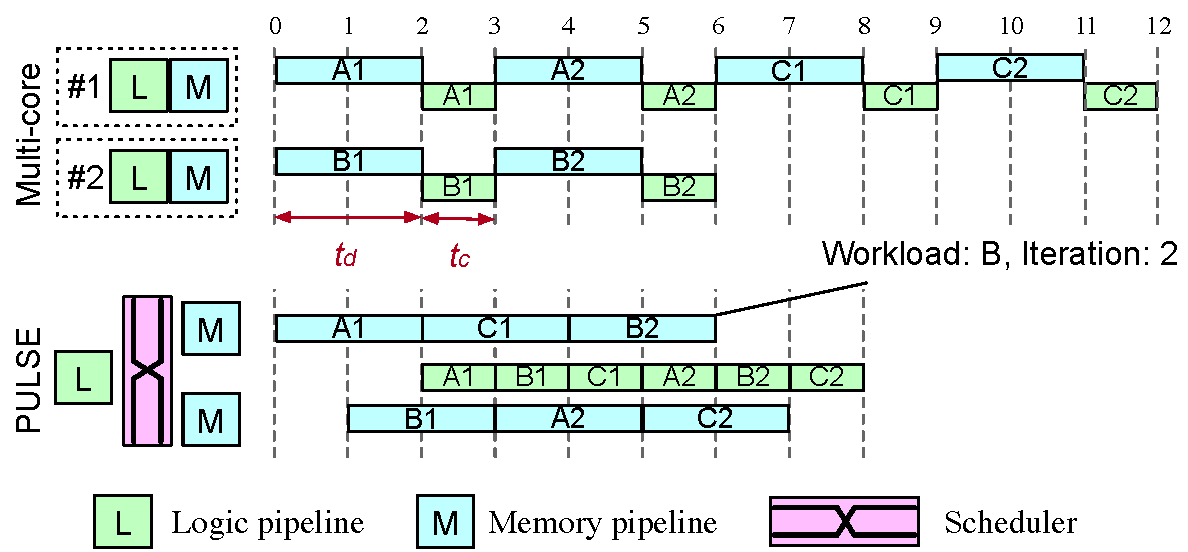
\includegraphics[width=0.7\columnwidth]{fig/pulse/architecture.pdf}
  \caption[\pulse accelerator architecture]{\textbf{\pulse accelerator architecture.} (top) Traditional multi-core architectures with tightly coupled logic and memory pipelines result in low utilization and longer execution times. (bottom) \pulse accelerator's \emph{disaggregated} design with an unequal number of logic and memory pipelines efficiently multiplexes concurrent iterator executions across them for near-optimal utilization and performance.}
  \label{fig:architecture_overview}
\end{figure} 

\paragraphb{Disaggregated accelerator design} Motivated by the unique characteristics of iterators, we propose a novel accelerator architecture that \emph{disaggregates memory and logic pipelines}, using a scheduler to multiplex iterator components across these pipelines. This decoupling enables an asymmetric number of logic and memory pipelines, maximizing the utilization of each, in contrast to the tightly coupled architecture of multi-core processors. In our design, if there are $m$ logic pipelines and $n$ memory pipelines, the accelerator-specific threshold $\eta < 1$ (as introduced in \S\ref{ssec:compute_node}) is given by $\eta = \frac{m}{n}$, meaning there are fewer logic pipelines than memory pipelines, consistent with Property 2. Fig.~\ref{fig:architecture_overview}~(bottom) illustrates an example of this disaggregated design with one logic pipeline and two memory pipelines ($m=1, n=2$).

Although data fetch and logic execution within each iterator must occur sequentially, the disaggregated architecture allows efficient multiplexing of data fetch and logic execution from different iterators across the separated pipelines, thus maximizing overall utilization. Recall that the logic execution time $t_c$ for each offloaded iterator execution in \pulse is constrained by $t_c \leq \eta \cdot t_d$, where $t_d$ is the time spent on data fetch (\S\ref{ssec:compute_node}). In the extreme case where $t_c = \eta \cdot t_d$ for all iterator executions, it becomes possible to multiplex $m+n$ concurrent iterator executions to fully utilize all $m$ logic and $n$ memory pipelines. While we omit the theoretical proof for brevity, Fig.~\ref{fig:architecture_overview}~(bottom) demonstrates the multiplexed execution—managed by a scheduler in our accelerator—for $t_c = \frac{1}{2} \cdot t_d$ using 3 iterators. This is the ideal case. Similar multiplexing is possible even when $t_c \leq \eta \cdot t_d$, fully utilizing the memory pipelines, though with lower utilization of logic pipelines (since they will be idle for a fraction of the time given by $\frac{t_c - \eta \cdot t_d}{t_c}$). Consequently, we provision $\eta = \frac{m}{n}$ to be as close as possible to the expected ratio $\frac{t_c}{t_d}$ for the workload to maximize the utilization of logic pipelines. Further improvements in logic pipeline energy efficiency can be achieved through dynamic frequency scaling~\cite{daepowerscaling}, though we leave such optimizations for future work.

While the memory pipeline is stateless, the logic pipeline must maintain the state for the iterator it is executing. To efficiently multiplex several iterator executions, the logic pipelines require mechanisms for fast context switching. Each iterator execution is associated with a dedicated \emph{workspace}, which stores three distinct pieces of state: \code{cur\_ptr} and \code{scratch\_pad}, which track the iterator state as described in \S\ref{ssec:pulseinterface}, and \code{data}, which holds the memory data loaded for \code{cur\_ptr}. Maintaining a dedicated workspace for each iterator allows the logic pipeline to switch between iterator executions without delay, as triggered by the scheduler. However, this requires maintaining multiple workspaces—up to $m+n$ to support all possible schedules, given our bound on the number of concurrent iterators. These workspaces are distributed evenly across the logic pipelines.



\begin{figure}[t]
\centering
  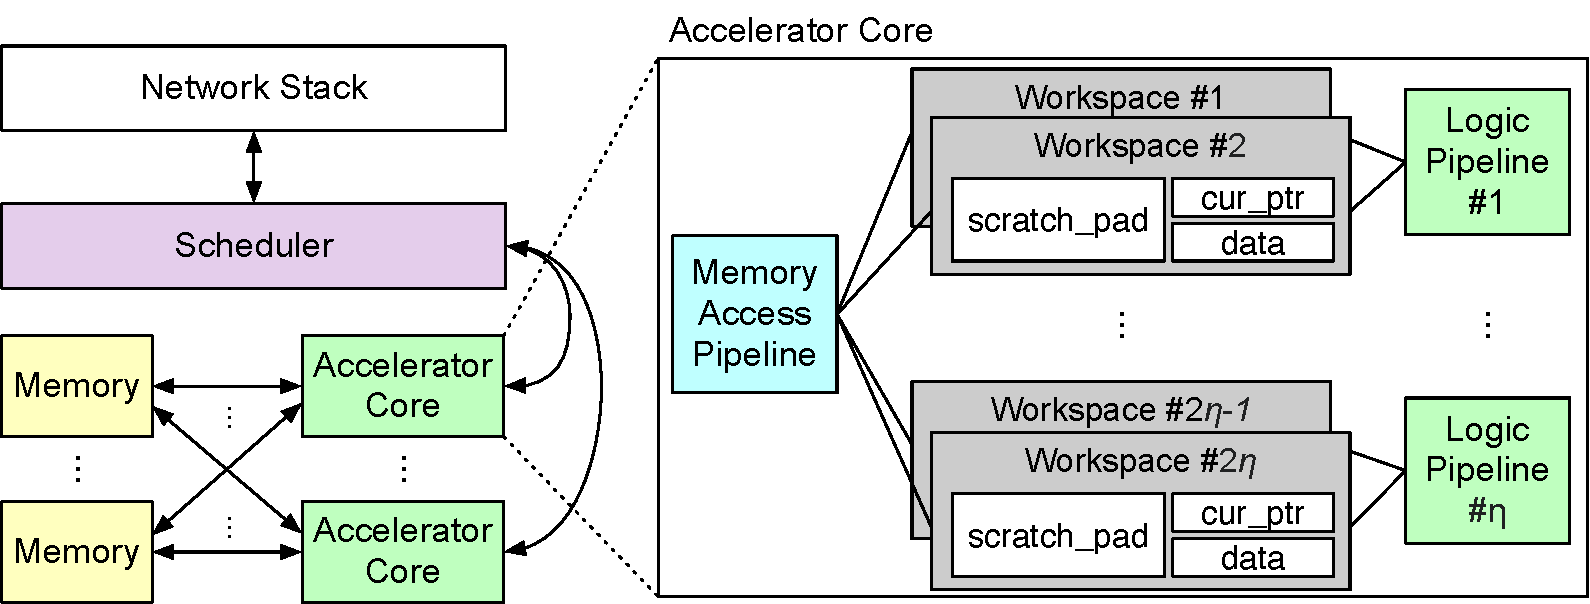
\includegraphics[width=0.7\columnwidth]{fig/pulse/accelerator.pdf}
 \caption[\pulse accelerator overview]{\textbf{\pulse accelerator overview.} See \S\ref{ssec:pulsearchitecture} for details.}
\label{fig:accelnew}
\end{figure}
\paragraphb{\pulse Accelerator Components} The \pulse accelerator consists of $n$ memory pipelines and $m$ logic pipelines for processing iterator requests, a scheduler that multiplexes these requests across the pipelines, and a network stack for handling pointer-traversal requests from the network (Fig.~\ref{fig:accelnew}).

\paragraphc{Memory pipeline:} Each memory pipeline loads data from the attached DRAM to the corresponding workspace, as assigned by the scheduler at the start of each iteration. This process involves (i) address translation and (ii) memory protection based on page access permissions. To optimize on-chip storage, we implement range-based address translations, previously simulated in prior work~\cite{range}, using TCAM.

Once a memory access is completed, the memory pipeline signals the scheduler to either continue the iterator execution or terminate it if a translation or protection failure occurs.

\paragraphc{Logic pipeline:} The logic pipeline executes all \pulse ISA instructions except for \code{LOAD}/\code{STORE}, determining the \code{cur\_ptr} value for the next iteration or checking whether the termination condition has been met. Each logic pipeline consists of an ALU for executing arithmetic and logic instructions, along with modules for register manipulation, branching, and executing the specialized \code{RETURN} instruction (Table~\ref{tab:isa}). During the execution of an iterator, the logic pipeline reads from and updates the registers in its dedicated workspace. An iteration can terminate in two ways: (i) the \code{cur\_ptr} is updated to the next pointer and the \code{NEXT\_ITER} instruction is reached, or (ii) the traversal completes and the \code{RETURN} instruction is reached. In either case, the logic pipeline sends the appropriate signal to the scheduler.

\paragraphc{Scheduler:} The scheduler coordinates the data fetch and logic execution for each iterator across the memory and logic pipelines:
\begin{enumerate}[leftmargin=*, itemsep=0pt]
  \item Upon receiving a new request over the network, the scheduler assigns the iterator to an empty workspace in a logic pipeline and signals one of the memory pipelines to perform the data fetch from memory based on the state stored in the workspace.\label{signal:1}
  \item After receiving a signal from the memory pipeline indicating that the data fetch has completed, the scheduler notifies the appropriate logic pipeline to continue the iterator execution using the corresponding workspace.
  \item When the logic pipeline signals that the next iteration can begin (via the \code{NEXT\_ITER} instruction), the scheduler signals one of the memory pipelines to execute the \code{LOAD} operation via the workspace.\label{signal:2}
  \item If the scheduler receives a signal from the memory pipeline about an address translation or memory protection failure, or a signal from the logic pipeline indicating the iterator execution has reached its termination condition (via the \code{RETURN} instruction), it signals the network stack to prepare a response containing the iterator \code{code}, \code{cur\_ptr}, and \code{scratch\_pad}.
\end{enumerate}
\noindent
The scheduler assigns memory and logic pipelines in steps~\ref{signal:1} and~\ref{signal:2} to maximize the utilization of all memory pipelines (as illustrated in Fig.~\ref{fig:architecture_overview}~(bottom)), though other scheduling policies could be implemented.

\paragraphc{Network Stack:} The network stack handles packet reception and transmission. When a new request arrives, it parses the payload to extract the request ID, \code{code}, and the state for the offloaded iterator execution (\code{cur\_ptr}, \code{scratch\_pad}). 

The network stack uses the same format for both requests and responses, allowing it to send a response back to the CPU node upon traversal completion or to reroute the request to another memory node for further execution (\S\ref{ssec:pulsedistributed}).

\paragraphb{Implementation} We implement \pulse on an FPGA-based NIC (Xilinx Alveo U250), which features two 100 Gbps Ethernet ports, 64 GB of on-board DRAM, 1,728K LUTs, and 70 MB of BRAM. The board's resources are partitioned into two \pulse accelerators, each utilizing one Ethernet port and two memory channels. Based on our analysis of common data structures (\S\ref{sec:pulseevaluation}), which shows that the $t_c/t_d$ ratio tends to be $< 0.75$, we configure $\eta = 0.75$. This results in four memory pipelines and three logic pipelines, with a total of $7$ workspaces per accelerator.

For efficient operation, we use Xilinx TCAM IP~\cite{tcam_ip} for page table management, 100 Gbps Ethernet IP, and link-layer IPs~\cite{xilinx_network}. Additionally, burst data transfers~\cite{burstdatatransfer} are employed to improve memory bandwidth. The logic and memory pipelines are clocked at 250 MHz, while the network stack operates at 322 MHz to handle 100 Gbps traffic. Although our current implementation demonstrates \pulse's capabilities on an FPGA prototype, we envision that the next logical step will be an ASIC implementation for even greater efficiency.

\subsection{Distributed Pointer Traversals}
\label{ssec:pulsedistributed}

Prior approaches to pointer traversals, which restrict them to a single memory node (\S\ref{sec:needforpulse}), force applications into two less-than-ideal choices. On one hand, applications can confine their data to a single memory node, limiting scalability. On the other hand, they can distribute data across multiple nodes, but each time a pointer on a different memory node is accessed, the traversal must return to the CPU node. This latter approach improves scalability but introduces additional network and software processing latency at the CPU node.

To bypass the overhead of returning to the CPU node, one could replicate the entire translation and protection state across all memory nodes, allowing them to directly forward traversal requests to other memory nodes. However, this strategy comes with increased space requirements for storing the translation state, which is difficult to accommodate within the limited capacity of the accelerator's translation and protection tables. Moreover, replicating this state across memory nodes introduces complexity, requiring protocols to maintain consistency when state changes occur—protocols that impose significant performance overheads.


\begin{figure}[t]
\centering
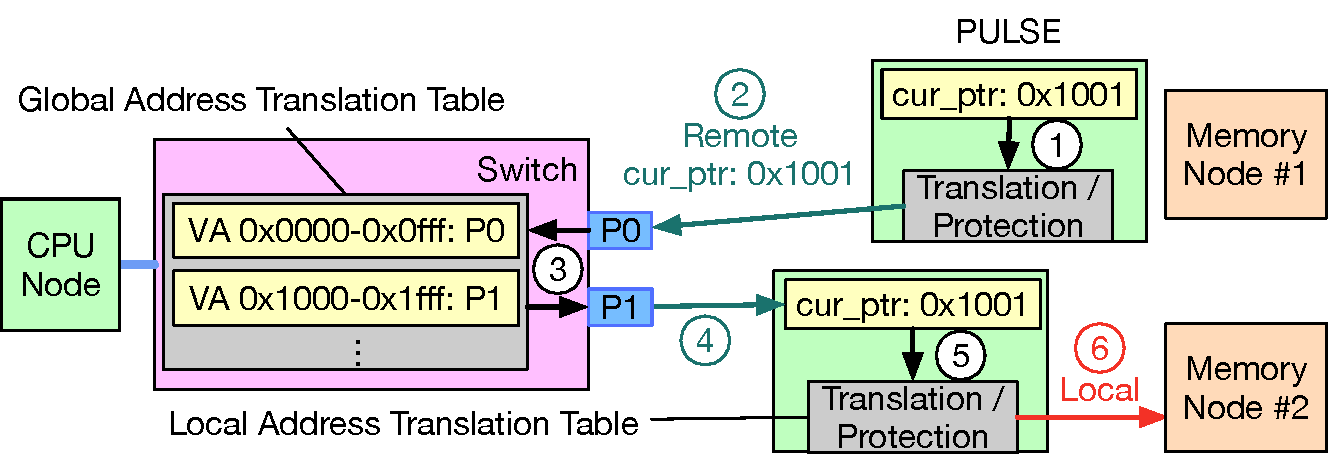
\includegraphics[width=0.7\columnwidth]{fig/pulse/hierarchical.pdf}
\caption[Hierarchical translation \& distributed traversal]{\textbf{Hierarchical translation \& distributed traversal (\S\ref{ssec:pulsedistributed}).}}
\label{fig:hierarchical}
\end{figure}

\pulse breaks the tradeoff between performance and scalability by utilizing a programmable network switch to enable rack-scale distributed pointer traversals. Specifically, when the \pulse accelerator at one memory node detects that the next pointer resides on a different memory node, it forwards the request to the network switch, which routes it to the correct memory node to continue the traversal. This approach reduces the network latency by half a round-trip time and eliminates the software overheads at the CPU node, as the routing logic is executed directly in the switch hardware. Since routing traversal requests across memory nodes is analogous to packet routing, the switch hardware is already optimized for this process.

However, enabling rack-scale pointer traversals introduces two key challenges, which we address next.

\paragraphb{Hierarchical translation} For the switch to forward a pointer traversal request to the correct memory node, it must determine which memory node is responsible for the relevant address. Given the limited resources at the switch, \pulse employs a hierarchical address translation mechanism, as illustrated in Fig.~\ref{fig:hierarchical}. 

The address space is range-partitioned across memory nodes, and only the base address-to-memory node mapping is stored at the switch. Each memory node, in turn, maintains its local address translation and protection metadata at the accelerator (\textcircled{1}), as described in \S\ref{ssec:pulsearchitecture}. The switch inspects the \code{cur\_ptr} field in the request (\textcircled{2}) and uses its base address mapping to identify the target memory node (\textcircled{3}). Once the request reaches the memory node, the traversal continues until a pointer is encountered that is not present in the local table (as in \textcircled{1}). At this point, the request is sent back to the switch (\S\ref{ssec:pulsearchitecture}), which can either re-route the request to another memory node (\textcircled{4}-\textcircled{6}) or notify the CPU node if the pointer is invalid.

\paragraphb{Continuing stateful iterator execution} A challenge in distributing iterator execution across memory nodes in \pulse is managing the stateful nature of the iterators. Since \pulse allows the storage of intermediate state in the iterator's \code{scratch\_pad}, how can the execution of such stateful iterators be seamlessly continued on a different memory node? Fortunately, the design choice of confining all iterator state within the \code{scratch\_pad} and \code{cur\_ptr}, coupled with the use of consistent request and response formats, makes this straightforward. The accelerator at the current memory node embeds the updated \code{scratch\_pad} in the response before forwarding it to the switch. When the switch forwards the request to the next memory node, execution continues exactly as if the previous memory node had the pointer.





\begin{figure*}[t]
\centering
  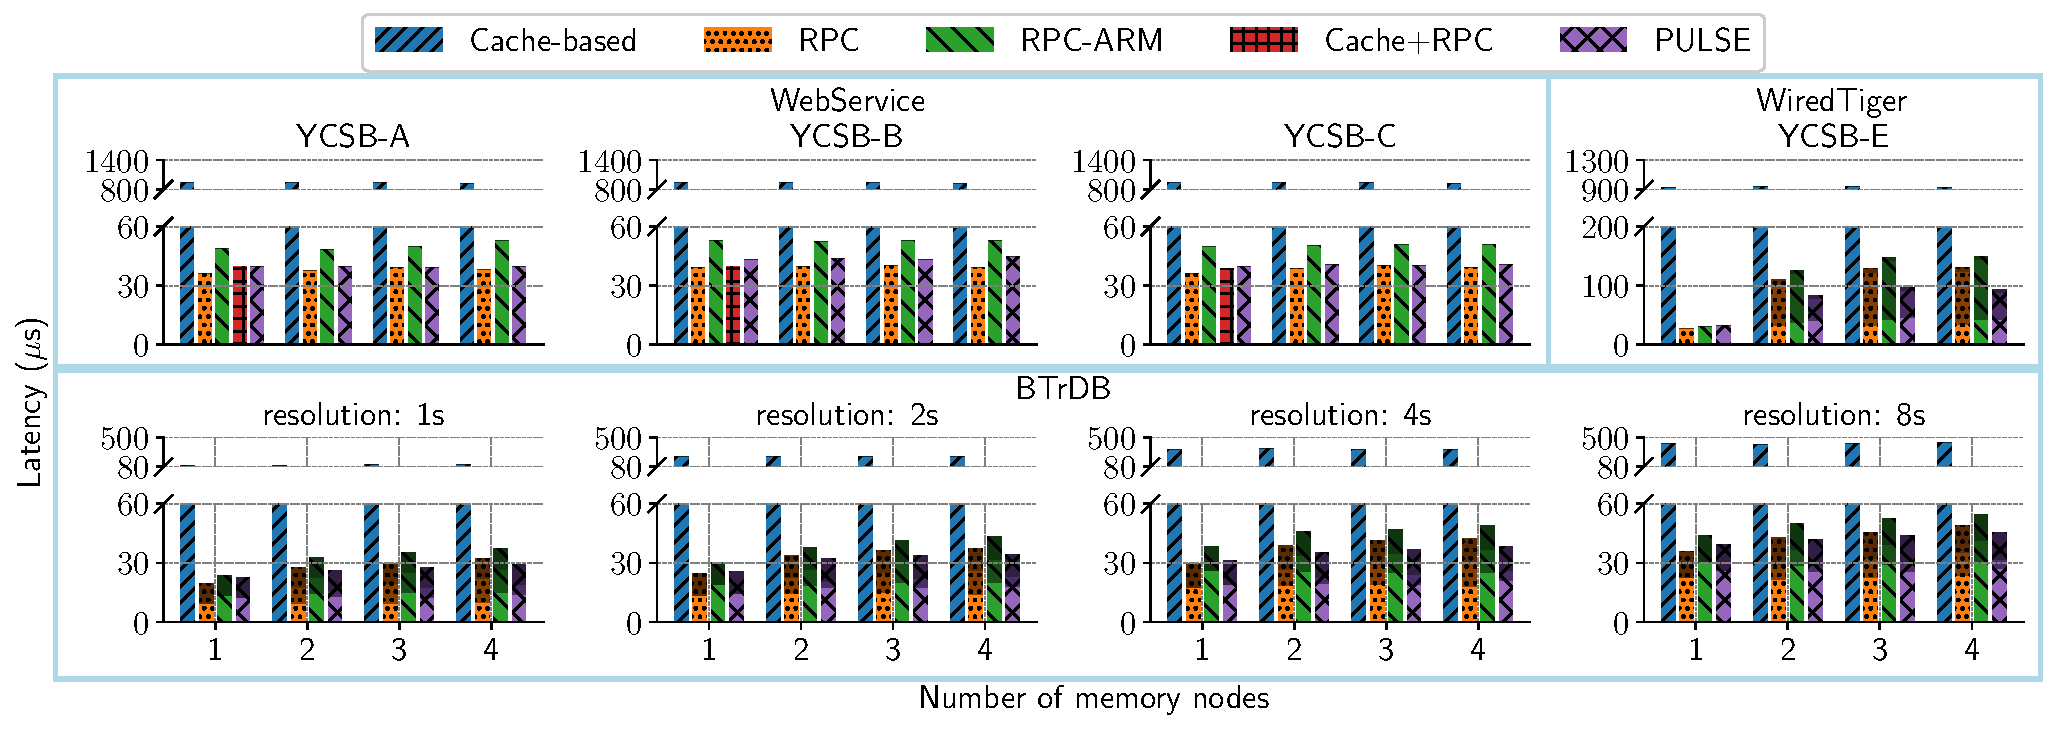
\includegraphics[width=\textwidth]{fig/pulse/latency.pdf}
  \\
  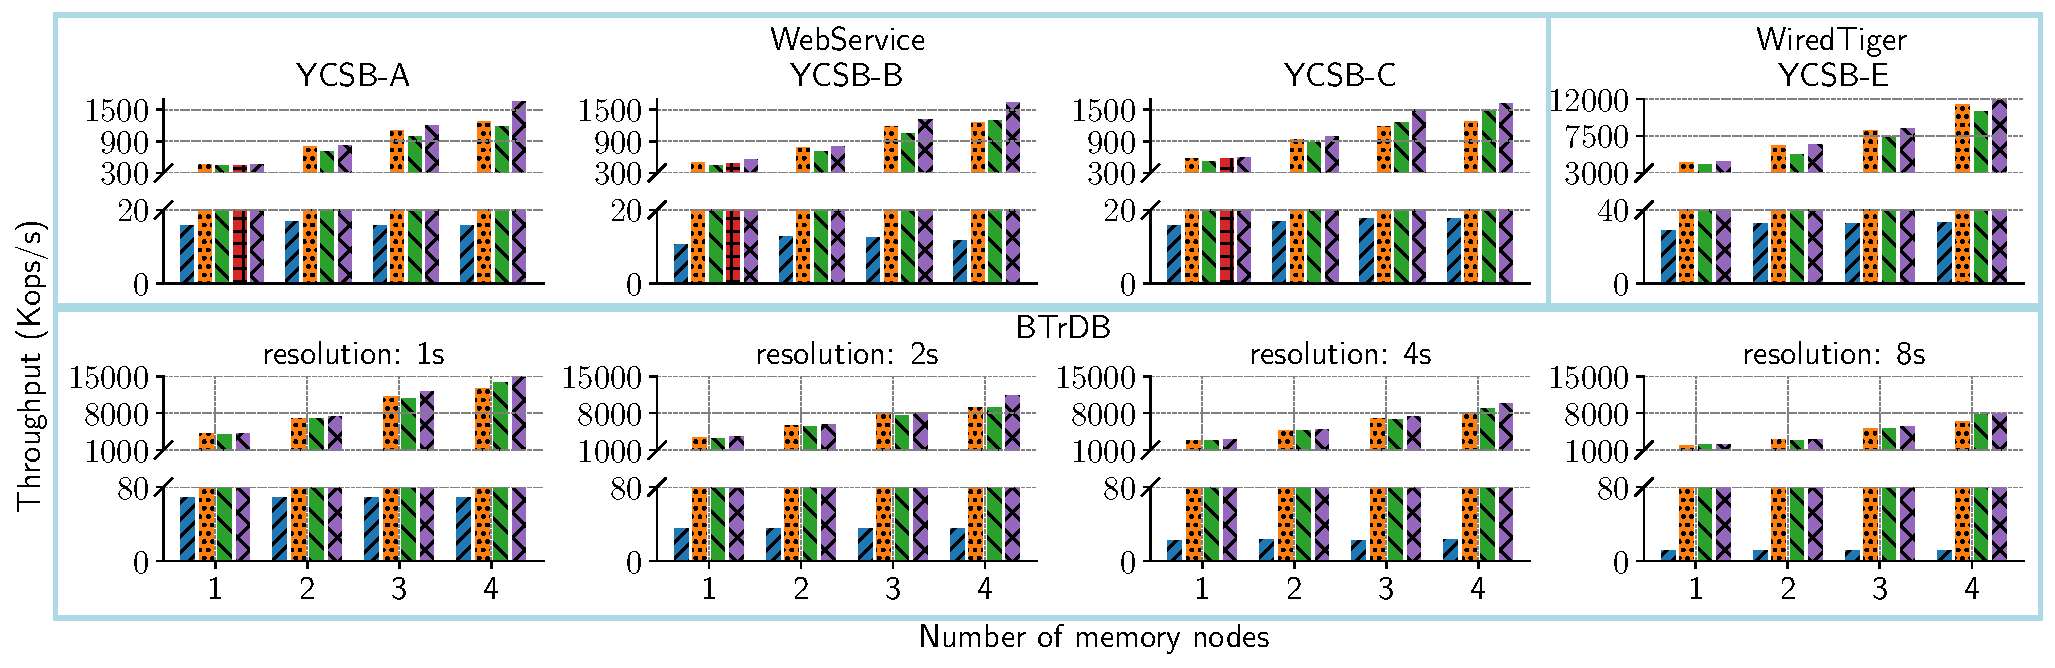
\includegraphics[width=\textwidth]{fig/pulse/throughput.pdf}
  \caption[Application latency \& throughput]{\textbf{Application latency (top) \& throughput (bottom) (\S\ref{ssec:pulseapplication-study}).} 
  The darker color indicates the time spent on cross-node pointer traversals, which increases with the number of memory nodes in WiredTiger and BTrDB.}
\label{fig:eval_perf_e2e_latency}
\label{fig:eval_perf_e2e_throughput}
\end{figure*}

\section{Evaluation}
\label{sec:pulseevaluation}



\paragraphb{Compared systems} We compare \pulse against the following systems: 
(1) a \textbf{Cache-based} system that relies solely on CPU node caches to accelerate remote memory accesses, using Fastswap~\cite{fastswap} as the representative system, 
(2) an \textbf{RPC} system that offloads pointer traversals to a CPU at the memory nodes, 
(3) \textbf{RPC-ARM}, an RPC system that employs wimpy ARM processors at the memory nodes, and 
(4) a \textbf{Cache$+$RPC} system that uses data structure-aware caches, represented by AIFM~\cite{aifm}. Systems (1) and (4) are configured with a cache size of $2$ GB, while systems (2) and (3) use a DPDK-based RPC framework~\cite{erpc}.

\paragrapha{Our experimental setup} consists of two servers—one acting as the CPU node and the other as the memory nodes—connected via a 32-port switch equipped with a $6.4$ Tbps programmable Tofino ASIC. Both servers are powered by Intel Xeon Gold 6240 processors~\cite{intelprocessor} and feature $100$ Gbps Mellanox ConnectX-5 NICs. 

To ensure a fair comparison, we limit the memory bandwidth of the memory nodes to $25$ GB/s, which corresponds to the peak bandwidth of the FPGA, using Intel Resource Director Technology~\cite{intel_cmt_cat}. We report the energy consumption based on the \textbf{minimum} number of CPU cores required to saturate the available bandwidth. For the ARM-based system (\textbf{RPC-ARM}), we use Bluefield-2 DPUs~\cite{bluefield}, which feature $8$ Cortex-A72 cores and $16$ GB of DRAM. 

For \pulse, we configure two memory nodes per FPGA NIC (one per port), resulting in a total of four memory nodes. The results from our experiments can be extrapolated to larger setups, as \pulse's performance and energy efficiency are independent of dataset size and cluster scale.


\begin{table}[!t]
  \centering
  \bgroup
  \small
  \def\arraystretch{0.95}%
  \begin{tabular}{l|c|c|c} 
        \hline
        \textbf{Application} & \textbf{Data Structure} & \textbf{$t_c/t_d$} & \textbf{\#Iterations} \\\hline\hline
        WebService & Hash-table & 0.06 & 48 \\\hline
        WiredTiger & \multirow{2}{*}{B+Tree} & 0.63 & 25 \\\cline{1-1}\cline{3-4}
        BTrDB ($1s$ to $8s$) & & 0.71 & $38$--$227$ \\\hline
  \end{tabular}
  \egroup
  \caption[Workloads used in our evaluation]{\textbf{Workloads used in our evaluation (\S\ref{sec:pulseevaluation}).} $t_c$ and $t_d$ correspond to compute and memory access time at the \pulse accelerator.} 
  \label{tab:workloads}
\end{table}

\paragraphb{Applications \& workloads} We consider $3$ applications with varying data structure complexity, compute/memory-access ratio, and iteration count per request (Table~\ref{tab:workloads}): (1) \textit{Web Service}~\cite{aifm} that processes user requests by retrieving user IDs from an in-memory hash table, using these IDs to fetch 8KB objects, which are then encrypted, compressed and returned to the user. Requests are generated using YCSB A (50\% read/50\% update), B (95\% read/5\% update), and C (100\% read) workloads with Zipf distribution~\cite{ycsb_workload}. (2) \textit{WiredTiger Storage Engine} (MongoDB backend~\cite{mongodb}) uses B+Trees to index NoSQL tables. Our frontend issues range query requests over the network to WiredTiger and plots the results. Similar to prior work~\cite{aifm, xrp}, we model user queries using the YCSB E workload with Zipf distribution~\cite{ycsb_workload} on $8$B keys and $240$B values. (3) \textit{BTrDB Time-series Database}~\cite{btrdb} is a database designed for visualizing patterns in time-series data. BTrDB reads the data from a B+Tree-based store for a given user query and renders the time-series data through an interactive user interface~\cite{mrplotter}. We run stateful aggregations (sum, average, min, max) for time windows of different resolutions, from $1$s to $8$s, on the Open $\mu$PMU Dataset~\cite{upmu} with voltage, current, and phase readings from LBNL’s power grid~\cite{btrdb}.




\subsection{Performance for Real-world Applications} 
\label{ssec:pulseapplication-study}


%We now evaluate the compared systems for real-world applications. 
Since AIFM~\cite{aifm} does not natively support B+-Trees or distributed execution, we restrict the Cache+RPC approach to the Web Service application on a single node.

\paragraphb{Single-node performance} Fig.~\ref{fig:eval_perf_e2e_latency} demonstrates the advantages of accelerating pointer-traversals at disaggregated memory. Compared to the Cache-based approach, \pulse achieves $9$--$34.4\times$ lower latency and $28$--$171\times$ higher throughput across all applications using only one network round-trip per request. RPC-based systems observe $1$--$1.4\times$ lower latency than \pulse due to their $9\times$ higher CPU clock rates. We believe an ASIC-based realization of \pulse has the potential to close or even overcome this gap. Cache$+$RPC incurs higher latency than RPC due to its TCP-based DPDK stack~\cite{ousterhout_shenango_19_nsdi, aifm} and does not outperform RPC, indicating that data structure-aware caching is not beneficial due to poor locality.

Latency depends on the number of nodes traversed during a single request and the response size. WebService experiences the highest latency due to large 8KB responses and long traversal length per request. In BTrDB, the latency increases (and the throughput decreases) as the window size grows due to the longer pointer traversals (see Table~\ref{tab:workloads}). Interestingly, the Cache-based approach performs significantly better for BTrDB than WebService and WiredTiger due to the better data locality in time-series analysis of chronologically ordered data. However, its throughput remains significantly lower than both \pulse and RPC since it is bottlenecked by the swap system performance, which could not evict pages fast enough to bring in new data. This is verified in our analysis of resource utilization (deferred to Appendix for brevity); we find that RPC, RPC-ARM, Cache$+$RPC, and \pulse can utilize more than 90\% of the memory bandwidth across the applications, while the Cache-based approach observes less than 1 Gbps network bandwidth. The other systems --- \pulse, RPC, RPC-ARM, and Cache$+$RPC --- can also saturate available memory bandwidth (around $25$ GB/s) by offloading pointer traversals to the memory node, consuming only 0.5\%--25\% of the available network bandwidth. 

\paragraphb{Distributed pointer traversals} Fig.~\ref{fig:eval_perf_e2e_latency} shows that employing multiple memory nodes introduces two major changes in performance trends: (1) the latency increases when the pointer traversal spans multiple memory nodes, and (2) throughput increases with the number of nodes since the systems can exploit more CPUs or accelerators. WebService is an exception to the trend: since the hash table is partitioned across memory nodes based on primary keys, the linked list for a hash bucket resides in a single memory node. 

\pulse observes lower latency than the compared systems due to in-network support for distributed pointer-traversals (\S\ref{ssec:pulsedistributed}). The latency increases significantly from one to two memory nodes for all systems since traversing to the next pointer on a different memory node adds $5$--$10~\mu$s network latency. Also, even across two memory nodes, a request can trigger multiple inter-node pointer traversals incurring multiple network round-trips; for WiredTiger and BtrDB, $10$\%--$30$\% of pointer traversals are inter-node. However, in-network traversals allow \pulse to reduce latency overheads by $33$--$98$\%, with $1.1$--$1.36\times$ higher throughput than RPC.



\paragraphb{Energy consumption} We compared energy consumed per request for \pulse and RPC schemes at a request rate that ensured memory bandwidth was saturated for both. We measure energy consumption using Xilinx XRT~\cite{xilinx_xrt} for \pulse (all power rails) and Intel RAPL tools~\cite{intel_rapl} for RPC on CPUs~\cite{intelprocessor} (CPU package and DRAM only). For RPC-ARM on ARM cores, since there is no power-related performance counter~\cite{armv8registers} or open-source tool available, we adapt the measurement approach from prior work~\cite{clio}. Specifically, we calculate the CPU package's energy using application CPU cycle counts and DRAM power using Micron's estimation tool~\cite{micron}. Finally, we conservatively estimate ASIC power using our FPGA prototype: we scale down the ASIC energy only for \pulse accelerator using the methodology employed in prior research~\cite{asicpower} while using the unscaled FPGA energy for other components (DRAM, third-party IPs, \etc). As such, we measure an \emph{upper bound} on \pulse and \pulseasic energy use, and a \emph{lower bound} for RPC, RPC-ARM, and Cache+RPC.

\begin{figure}[t]
\centering
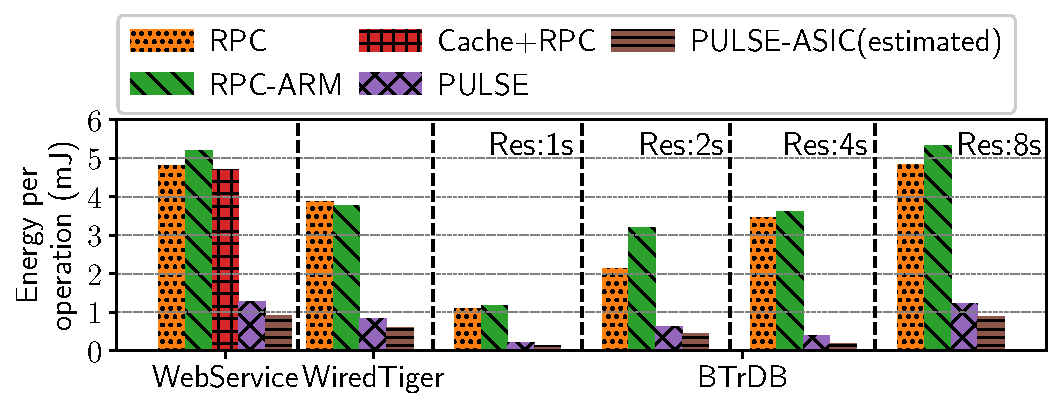
\includegraphics[width=0.8\textwidth]{fig/pulse/power.pdf}
\caption[Application energy consumption per operation]{\textbf{Application energy consumption per operation (\S\ref{ssec:pulseapplication-study}).}}
\label{fig:eval_energy}
\end{figure}

Fig.~\ref{fig:eval_energy} shows that \pulse achieves a $4.5$--$5\times$ reduction in energy use per operation compared to RPCs on a general-purpose CPU, due to its disaggregated architecture (\S\ref{ssec:pulsearchitecture}). Our estimation shows that \pulse's ASIC realization can conservatively reduce energy use by an additional $6.3-7\times$ factor. 
Finally, RPC-ARM's total energy consumption per request can exceed that of standard cores, as seen in the WebService workload. This observation aligns with prior studies~\cite{clio}, which attribute the increased energy use to their longer execution times, resulting in higher aggregate energy demands.

\begin{figure}[t]
\centering
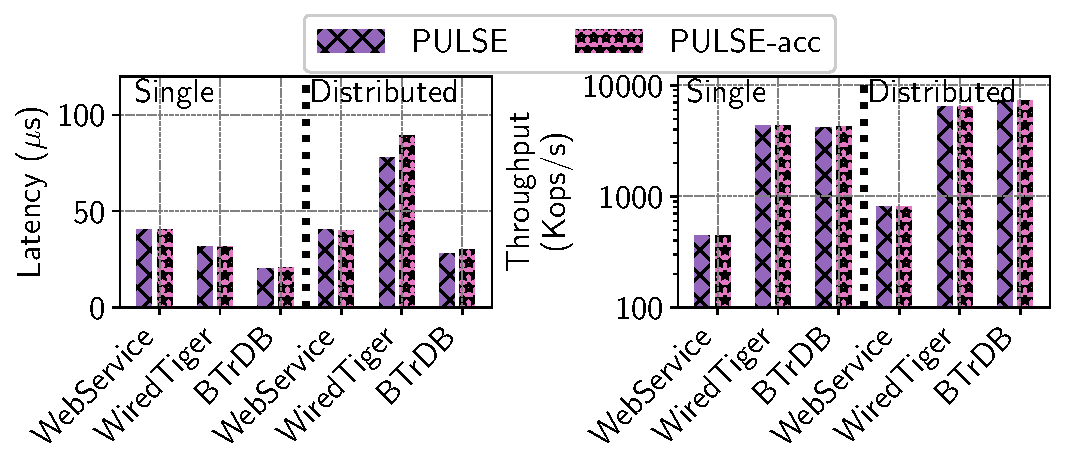
\includegraphics[width=0.8\textwidth]{fig/pulse/breakdown.pdf}%
\caption[Impact of distributed pointer traversals]{\textbf{Impact of distributed pointer traversals (\S\ref{ssec:pulsebreakdown}).}}
\label{fig:eval_breakdown}
\end{figure}

\begin{figure}[t]
  \centering	
  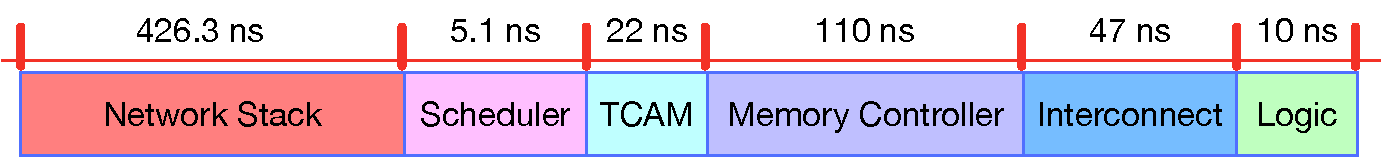
\includegraphics[width=0.8\textwidth]{fig/pulse/breakdown_latency_new.pdf}
  \caption[Latency breakdown for \pulse accelerator ]{\textbf{Latency breakdown for \pulse accelerator (\S\ref{ssec:pulsebreakdown}).}}
  \label{fig:eval_breakdown_latency_}
\end{figure}




\subsection{Understanding \pulse Performance}
\label{ssec:pulsebreakdown}




\paragraphb{Distributed pointer traversals} We evaluate the impact of distributed pointer traversals (\S\ref{ssec:pulsedistributed}) by comparing \pulse against \pulseacc, a \pulse variant that sends requests back to the CPU node if the next pointer is not found on the memory node. Fig.~\ref{fig:eval_breakdown} shows that while both have identical performance on a single memory node, \pulseacc observes $1.02$--$1.15\times$ higher latency for two nodes. On the other hand, their throughput is the same since, under sufficient load, memory node bandwidth bottlenecks the system for both.


\paragraphb{Latency breakdown for \pulse accelerator} 
Fig.~\ref{fig:eval_breakdown_latency_} shows the latency contributions of various hardware components at the \pulse accelerator for the WebService application. The network stack first processes the pointer traversal request in about $430$ ns, after which the WebService payload is processed by the scheduler and dispatched to an idle memory access pipeline in $5.1$ ns. Then, the memory pipeline takes $\sim$$132$ ns to perform address translation, memory protection, and data fetch from DRAM. Finally, the logic pipeline takes $10$ ns to check the termination conditions and determine the next pointer to look up. This process repeats until the termination condition is met. The time to send a response back over the network stack is symmetric to the request path.












\begin{figure}[t]
\centering
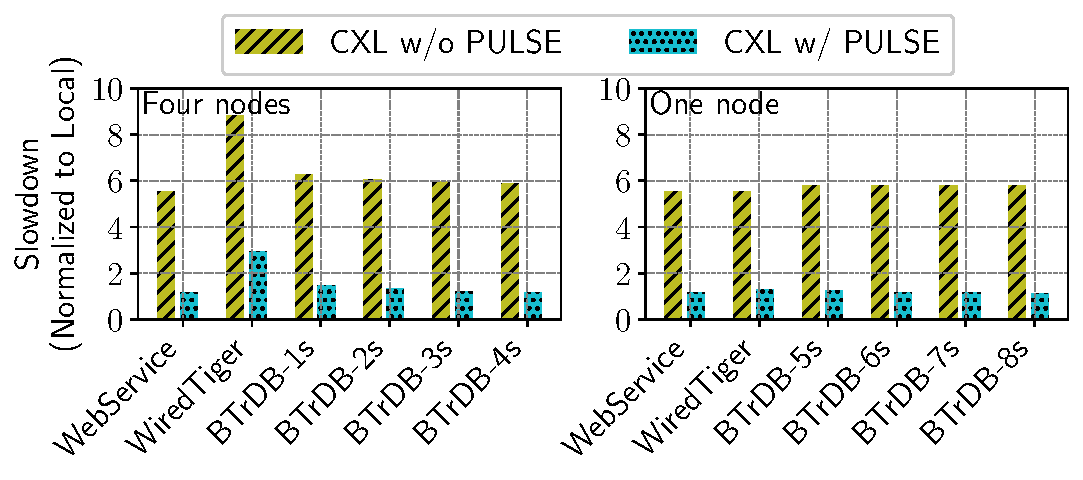
\includegraphics[width=0.9\columnwidth]{fig/pulse/cxl.pdf}
\caption[Slowdown with simulated CXL interconnect]{\textbf{Slowdown with simulated CXL interconnect.} }

\label{fig:eval_cxl}
\end{figure}

While \pulse is implemented atop Ethernet, its design is interconnect-agnostic and could be realized in ASIC-based or FPGA-attached memory devices over emerging interconnects like CXL~\cite{cxl, cxl_azure, sun2023demystifying}. We have verified these benefits in simulation atop detailed memory access and processing traces of our evaluated applications and workloads. The simulator maintains $2$GB of cache in local (CPU-attached) DRAM, while the entire working set is stored on remote CXL memory. Following prior work~\cite{pond}, we model $10$--$20$ns L3 cache latency, $80$ns local DRAM latency, $300$ns CXL-attached memory latency, and $256$B access granularity. We simulate both a four-memory-node setup, which uses a CXL switch with \pulse logic and a \pulse accelerator at each memory node, and a single-node setup with no switch. We assume a conservative overhead for \pulse, using our hardware programmable Ethernet switch and FPGA accelerator latencies.
 
 
Fig.~\ref{fig:eval_cxl} shows the average slowdown for executing our evaluated workloads on CXL memory relative to running it completely locally (\ie, the entire application working set fits in local DRAM) --- with and without \pulse. In the four-node setup, \pulse reduces CXL's slowdown by $19$--$33$\% across all applications. 

In the single-node setup, \pulse still reduces the slowdown by $19$--$23$\% by minimizing high-latency traversals over the CXL interconnect. While a real hardware realization is necessary to precisely quantify \pulse's benefits, our simulation (which models the lowest possible CXL latency and highest possible \pulse overheads) highlights its potential for improving performance in emerging interconnects.

\begin{figure*}[t]
\centering
  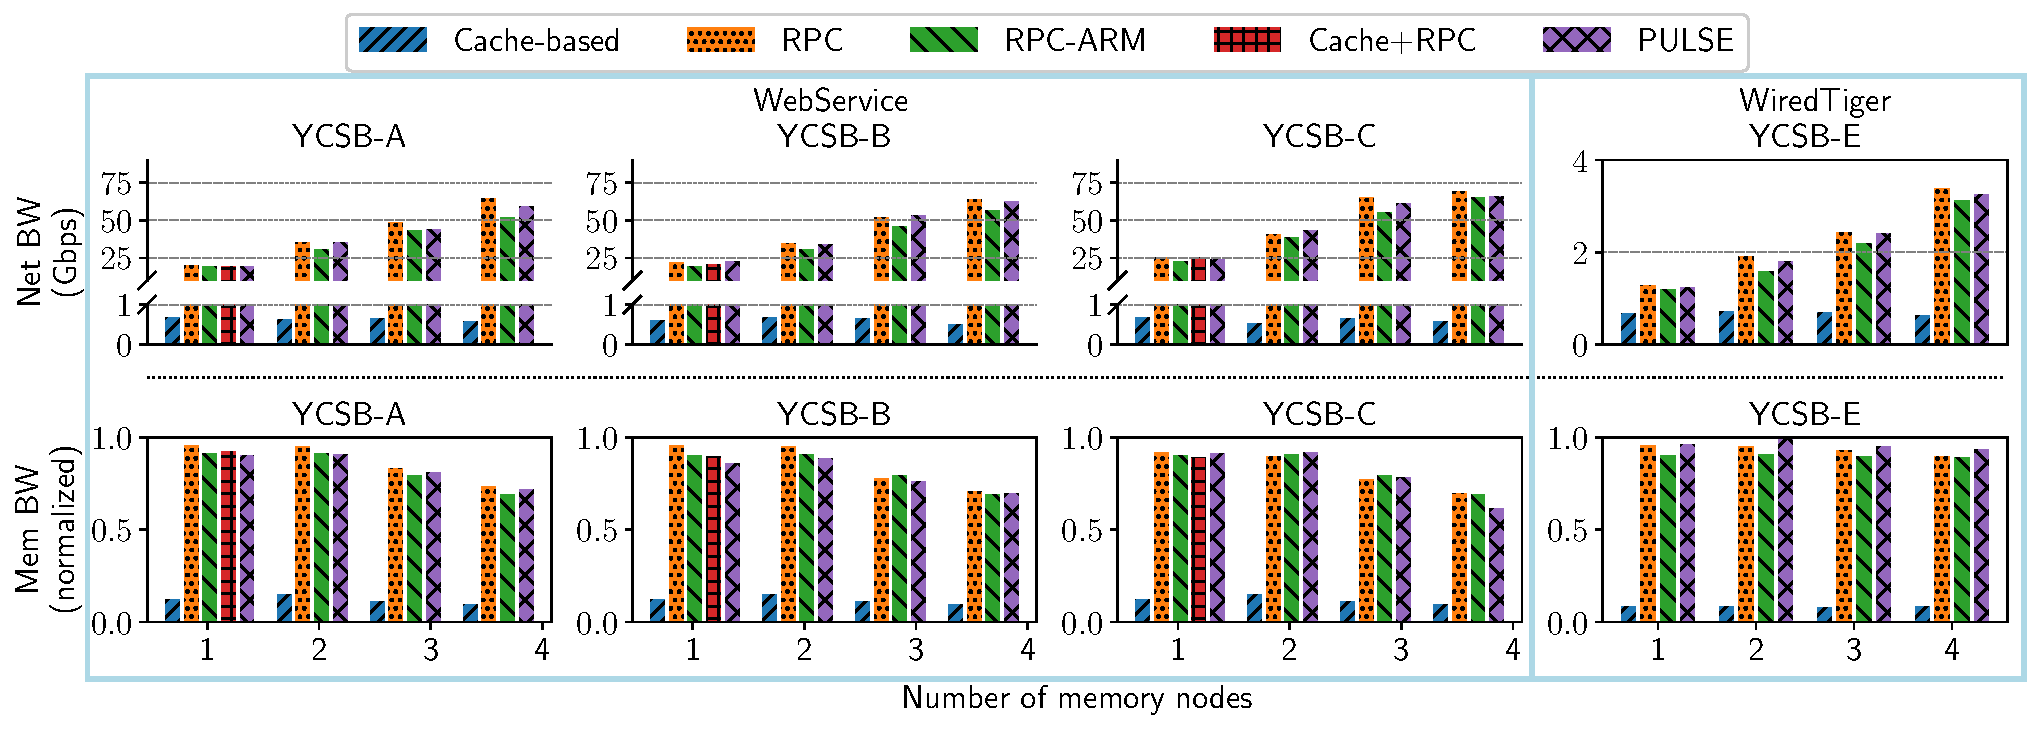
\includegraphics[width=\textwidth]{fig/pulse/network_memory.pdf}
  \caption[Network and memory bandwidth utilization]{\textbf{Network and memory bandwidth utilization.} \pulse and RPC utilize over 90\% of the available memory bandwidth, while the cache-based approach suffers from swap system overhead. In Webservice, the network bandwidth becomes the bottleneck due to large 8 KB data transfers.}
\label{fig:sup_eval_perf_e2e_utilization}
\end{figure*}

\subsection{Traditional Core Architecture vs. \pulse} 
We evaluate the impact of the \pulse architectural design (\S\ref{ssec:pulsearchitecture}) by comparing \pulse against \pulsearch, an in-order processor built on \pulse's components. We denote \textit{C\_x} as in tightly-coupled core architecture, where \textit{x} is the number of cores. We denote \textit{P\_x\_y} as \pulse architecture, where \textit{x} is the number of logic pipelines and \textit{y} is the number of memory pipelines. Table \ref{table:sup_architecture} shows the power, performance, and area usage of various configurations. The performance metrics are obtained by executing the WebService application with various configurations. In \pulse's disaggregated architecture, when the number of logic and memory pipelines is equal to that of a traditional core architecture, power and area usage are higher due to additional logic and buffering in the interconnect and scheduler. However, due to the nature of pointer traversal operations (\S\ref{ssec:pulsearchitecture}), \pulse requires fewer logic pipelines to achieve similar performance. For example, to fully saturate the memory bandwidth of a single node, \pulse uses only one logic pipeline and four memory pipelines, while a traditional core architecture requires four cores. As a result, \pulse saves 20.12\% in power with only a 7.2\% latency overhead, primarily due to the additional scheduler and data movement between workspaces.

\begin{table}[ht]
\centering
\scriptsize % Sets the font size to small to fit the table in a single column
\begin{tabularx}{0.6\columnwidth}{@{}Xcccccc@{}} % Adjust column types as needed
\toprule
\textbf{Config} & \textbf{Pwr (W)} & \textbf{LUT \%} & \textbf{BRAM \%}  & \textbf{Tpt (Mops/s)}   & \textbf{Lat (us)} \\
\midrule
C\_1 & 67.76 & 14.73 & 14.57 & 0.41 & 33.25   \\
C\_2 & 75.47 & 20.46 & 18.73 & 0.63 & 33.73   \\
C\_3 & 84.57 & 28.66 & 31.83 & 0.87 & 34.66   \\
C\_4 & 89.77 & 37.10 & 34.17 & 1.20 & 35.11  \\
P\_1\_1 & 56.74 & 11.76 & 16.34 & 0.51 & 37.57 \\
P\_1\_2 & 59.47 & 14.87 & 18.38 & 0.73 & 36.74 \\
P\_1\_3 & 64.78 & 16.64 & 22.37 & 1.01 & 38.46 \\
P\_1\_4 & 72.47 & 18.37 & 25.84 & 1.24 & 38.37 \\
P\_2\_1 & 67.37 & 17.73 & 20.37 & 0.48 & 40.27 \\
P\_2\_2 & 77.37 & 21.38 & 22.38 & 0.76 & 39.47 \\
P\_2\_3 & 81.21 & 26.22 & 26.76 & 0.99 & 41.37 \\
P\_3\_3 & 86.15 & 37.21 & 30.12 & 1.03 & 40.98 \\
P\_2\_4 & 83.21 & 30.13 & 31.21 & 1.19 & 40.37 \\
P\_4\_4 & 95.64 & 46.42 & 39.84 & 1.21 & 41.47\\
\bottomrule
\end{tabularx}
\caption{Comparison between traditional core architecture and \pulse architecture.}
\label{table:sup_architecture}
\end{table}




\begin{figure}[t]
\centering
\subfigure[Impact of access pattern]{
  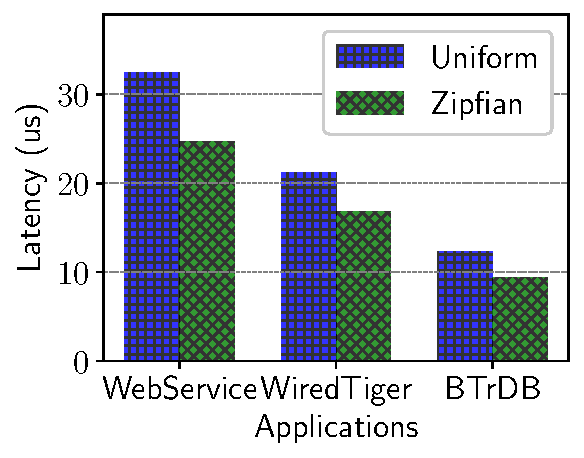
\includegraphics[width=0.4\columnwidth]{fig/pulse/micro_cache_friendly.pdf}
  \label{fig:sup_cache_friendly}}
\subfigure[Impact of modifications]{
  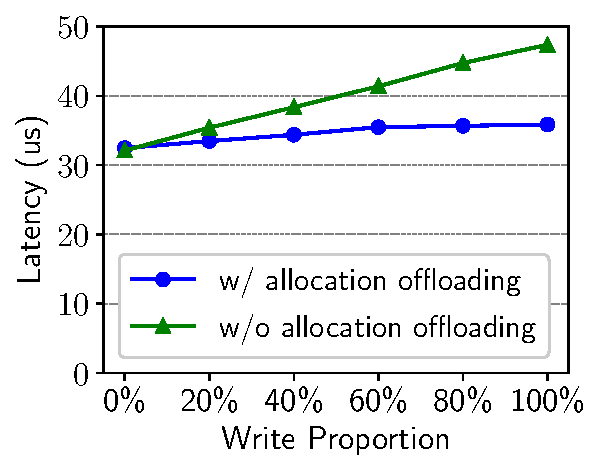
\includegraphics[width=0.4\columnwidth]{fig/pulse/micro_write.pdf}
  \label{fig:sup_write}}
\caption[Impact of access pattern and modifications]{(a) \pulse latency is up to $1.3\times$ lower for skewed than uniform access patterns due to caching. (b) Offloaded allocations in \pulse improve the WebService request latencies as the proportion of writes increases by reducing the number of round trips per allocation.}
\label{fig:sup_eval_cache_friendly}
\end{figure}

\begin{figure}[!ht]
    \centering
    \subfigure[Traversal length]{
        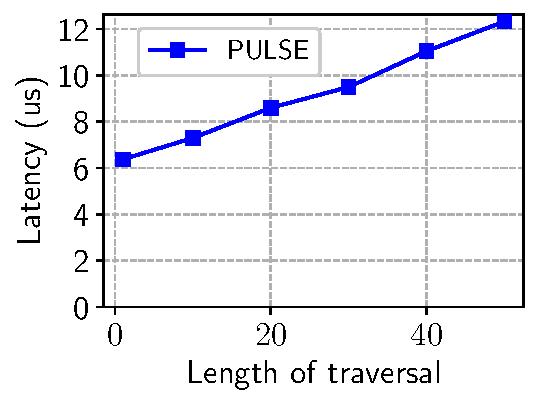
\includegraphics[width=0.4\columnwidth]{fig/pulse/sensitivity_length.pdf}
        \label{fig:sup_eval_sensitivity_length}    
    }%
    \subfigure[Number of memory pipelines]{
        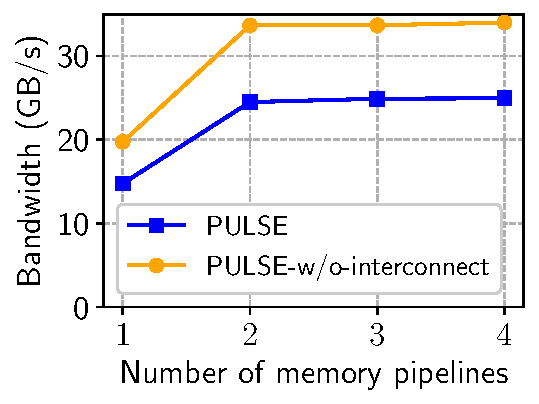
\includegraphics[width=0.4\columnwidth]{fig/pulse/sensitivity_core.pdf}
        \label{fig:sup_eval_sensitivity_core}
    }
    \caption[Sensitivity to traversal length and the number of memory pipelines]{\textbf{Sensitivity to traversal length and the number of memory pipelines.} (a) \pulse latency scales linearly with the length of traversal. (b) \pulse accelerator can saturate memory bandwidth with just two \pulse memory pipelines.}
\end{figure}
    

\begin{figure}[b]
\centering
  \subfigure[Latency]{
    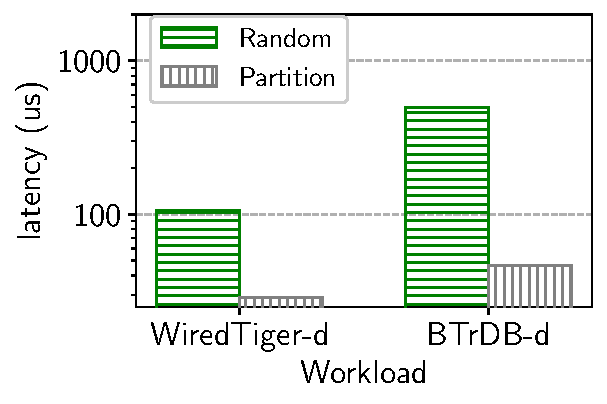
\includegraphics[width=0.4\columnwidth]{fig/pulse/sensitivity_allocation_latency.pdf}
    \label{fig:sup_eval_sensitivity_allocation_latency}
  }%
  \subfigure[Throughput]{
    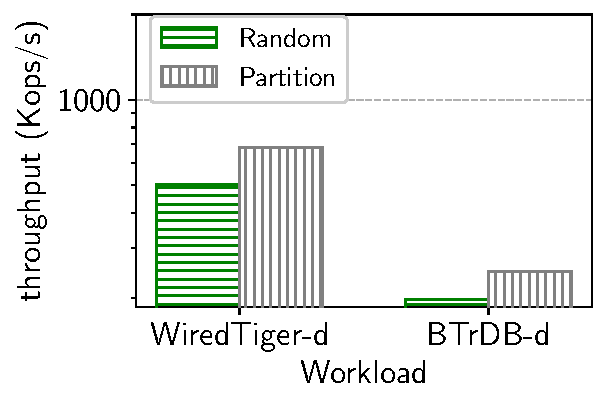
\includegraphics[width=0.4\columnwidth]{fig/pulse/sensitivity_allocation_throughput.pdf}
    \label{fig:sup_eval_sensitivity_allocation_throughput}
  }%
  \caption[Allocation policy]{\textbf{Allocation policy.} \pulse performs better with the partitioned allocation since it minimizes cross-node traversals.}
\end{figure}


\subsection{Network and Memory Bandwidth Utilization} 
We evaluate the network and memory bandwidth utilization of the three applications in Fig. \ref{fig:sup_eval_perf_e2e_utilization}. For WiredTiger, \pulse and RPC utilize over 90\% of the available memory bandwidth, while the Cache-based approach suffers from low network bandwidth and memory utilization due to swap system overhead. For WebService, the large 8 KB data transfers saturate the maximum bandwidth that the DPDK stack can sustain~\cite{erpc}. As a result, network bandwidth becomes the bottleneck, reducing \pulse and RPC memory bandwidth utilization under 3 and 4 memory nodes. The memory bandwidth is normalized, where $1.0$ corresponds to $25$ GB/s per node.



\begin{figure*}[t]
\centering
  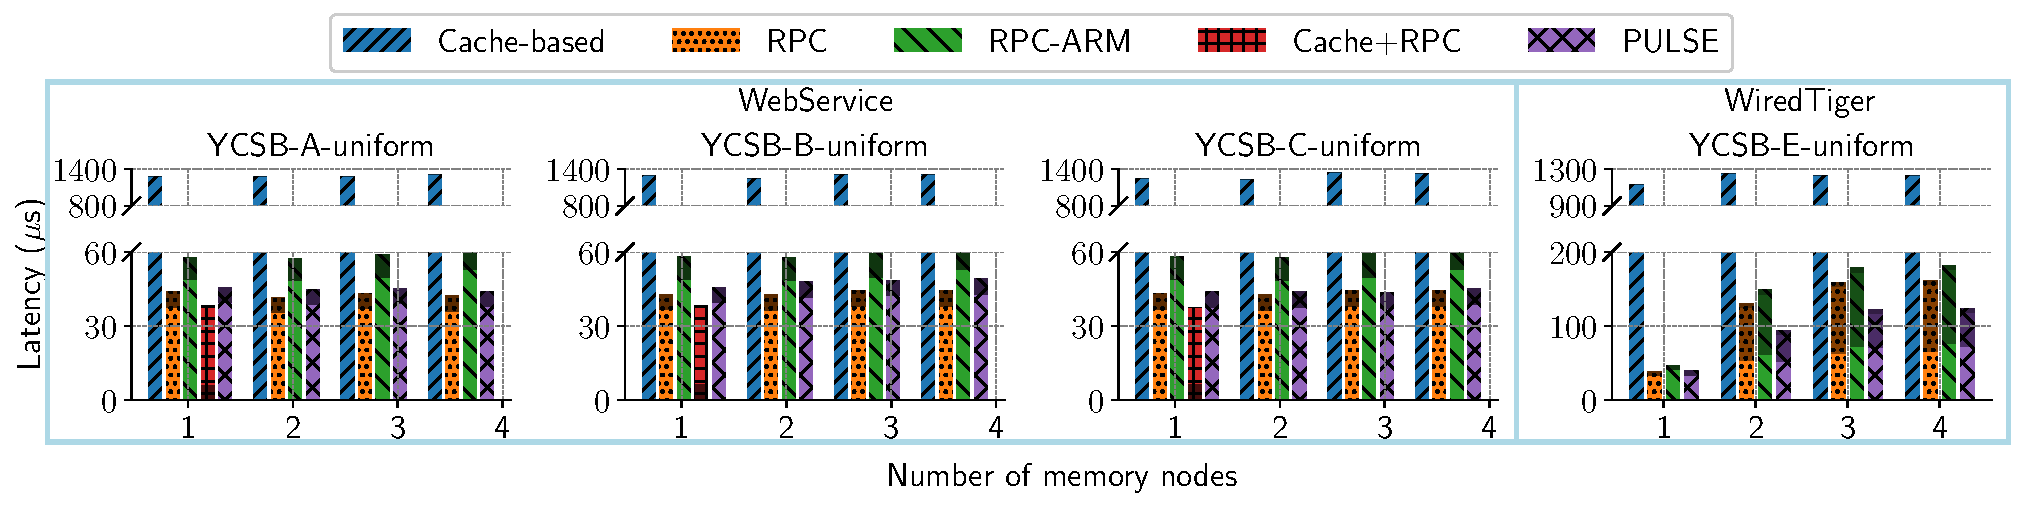
\includegraphics[width=\textwidth]{fig/pulse/latency_uniform.pdf}
  \label{fig:sup_eval_perf_e2e_latency_uniform}
  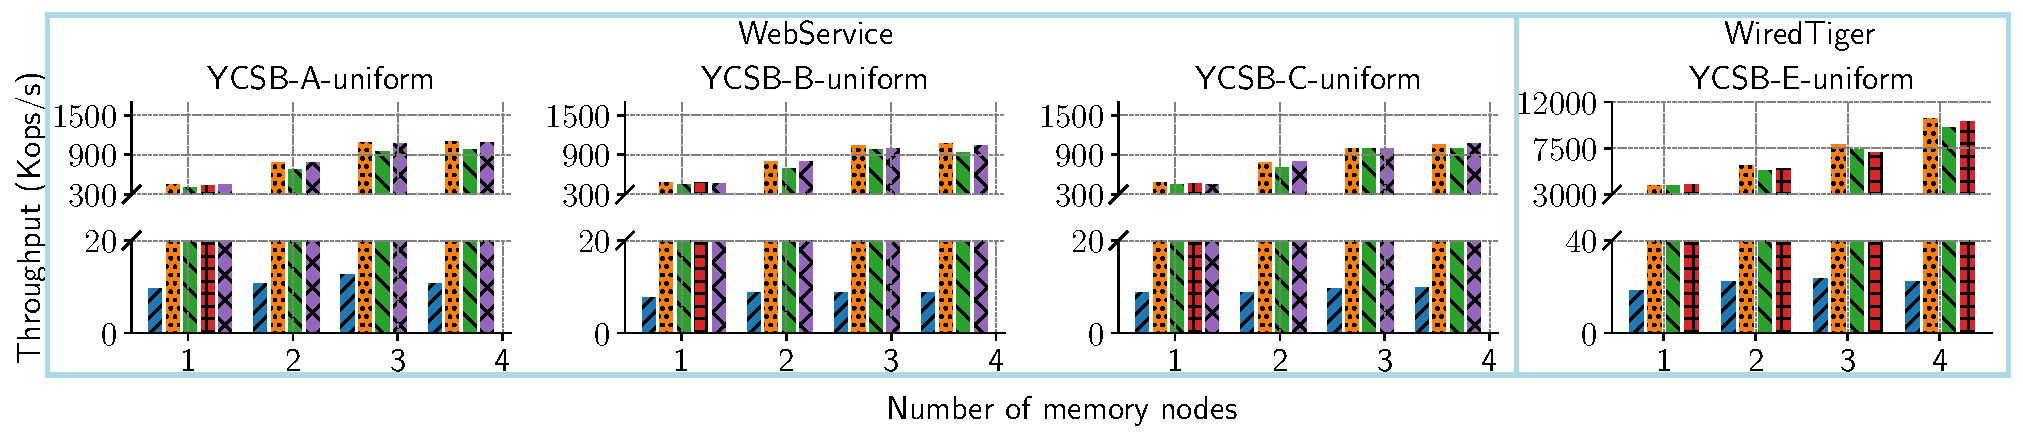
\includegraphics[width=\textwidth]{fig/pulse/throughput_uniform.pdf}
  \label{fig:sup_eval_perf_e2e_throughput_uniform}
  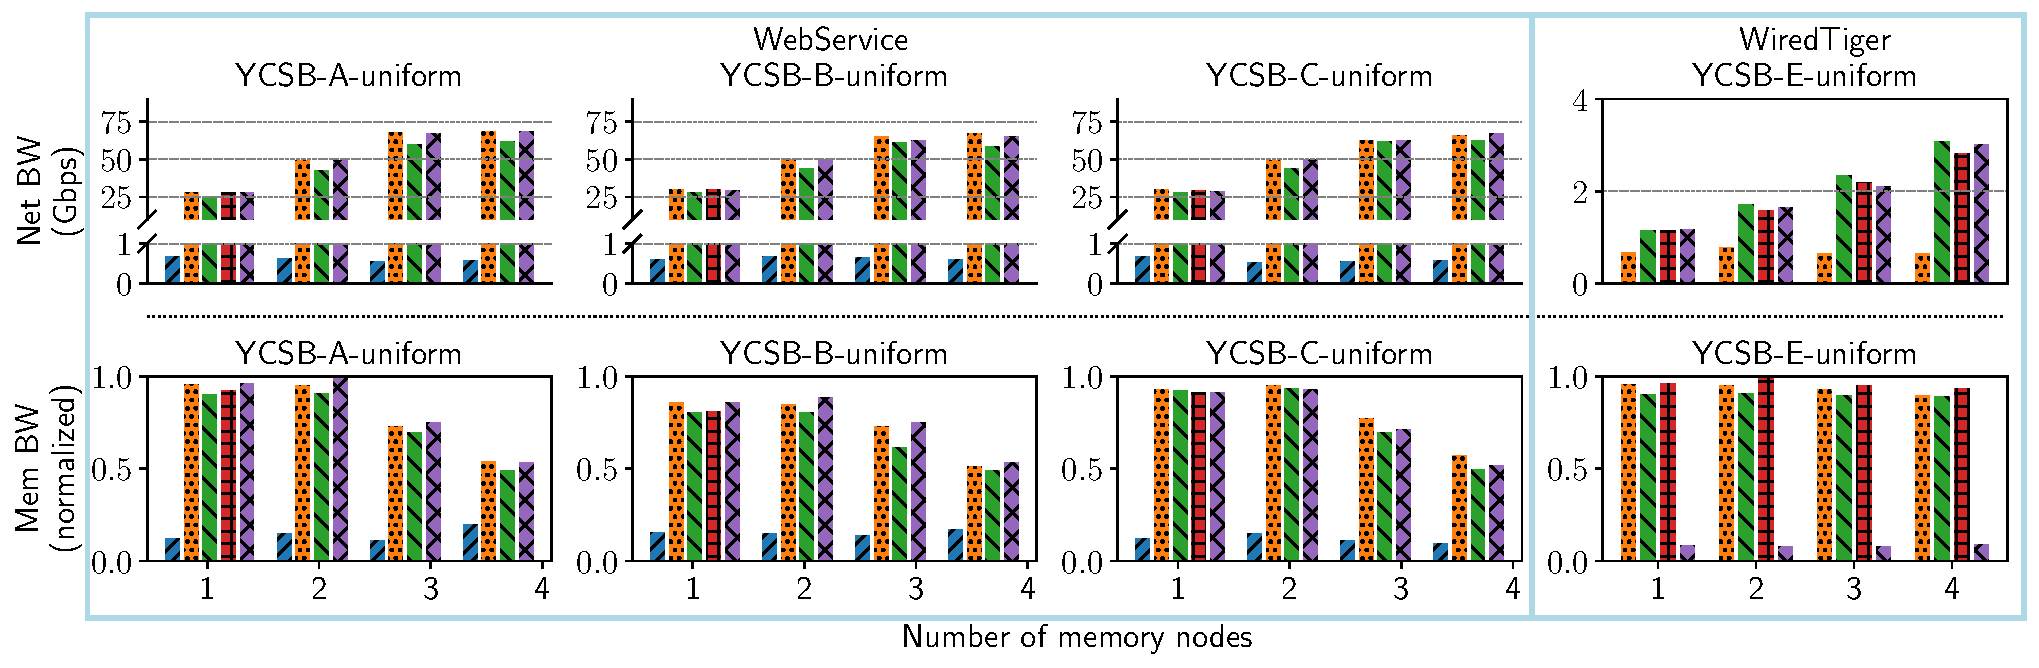
\includegraphics[width=\textwidth]{fig/pulse/network_memory_uniform.pdf}
  \label{fig:sup_eval_perf_e2e_utilization_uniform}
  \caption[Application performance using workload with uniform distribution]{\textbf{Application performance using workload with uniform distribution.}}
  \label{fig:sup_eval_uniform}

\end{figure*}


\subsection{\pulse Sensitivity Analysis}
\label{ssec:pulsesensitivity}


We evaluate \pulse's sensitivity to workload characteristics and system parameters: access pattern, data structure modifications, traversal length, allocation policy, and the number of \pulse memory pipelines. 


\paragraphb{Impact of access pattern}
While our evaluation so far has been confined to Zipfian workloads, we evaluate the impact of skewed access patterns on \pulse performance for all three applications. Our setup comprises a single $32$GB memory node with a $2$GB CPU node cache. Figure~\ref{fig:sup_cache_friendly} shows caching at the CPU node reduces the number of iterator requests offloaded to the \pulse accelerator for the skewed (Zipfian) workload, improving \pulse performance for such workloads by up to $1.33\times$ relative to uniform ones.

\paragraphb{Impact of data structure modifications} Operations that modify data structures can require new memory allocations during traversal. Instead of returning control to the CPU node for allocations, \pulse populates the scratchpad for every request with a fixed number of pre-allocated memory regions. When a new allocation is initiated at the \pulse accelerator, it uses a pre-allocated memory region on the scratchpad. If all such regions ($16$ in our implementation) are used up in a single request, the traversal interrupts and returns to the CPU node. \pulse periodically replenishes pre-allocated entries, ensuring that allocation-triggered traversal interruptions are rare.

We evaluate the impact of data structure modifications in \pulse by increasing the proportion of writes for the WebService application on a single memory node. Figure~\ref{fig:sup_write} shows that as the proportion of writes increases, \pulse without offloaded allocations experiences higher latencies (up to $1.4\times$) since each new node allocation requires two additional round trips; offloaded allocations reduce the allocation overhead to $<1.1\%$.

\paragraphb{Length of traversal} For simplicity, we evaluate traversal queries on a single linked list with varying numbers of nodes traversed per query. As expected, Fig.~\ref{fig:sup_eval_sensitivity_length} shows that the end-to-end execution latency for a linked list traversal scales linearly with the number of nodes traversed.

\paragraphb{Allocation policy} We find that the allocation policy used for a data structure has a significant impact on application performance specifically for distributed traversals (Figs.~\ref{fig:sup_eval_sensitivity_allocation_latency} and~\ref{fig:sup_eval_sensitivity_allocation_throughput}). We evaluated the WiredTiger and BTrDB workloads (that employ B+-Tree as their underlying data structure) with two allocation policies: one that partitions allocations in a way that ensures all nodes in half the subtree are placed on one memory node and the other half on another, and another that allocates memory uniformly across the two nodes (as in \code{glibc} allocator). The average latency for random allocations is $3.7-10.8\times$ higher than partitioned allocation since it incurs significantly more cross-node traversals. This shows that while uniformly distributed allocations can enable better system-wide resource utilization, it may be preferable to exploit application-specific partitioned allocations for workloads where performance is the primary concern. 

\paragraphb{Number of \pulse memory pipelines} We evaluate the number of \pulse memory access pipelines required to saturate \pulse's memory bandwidth on a single memory node. We used the same linked list as our traversal-length experiment due to its relatively low $\eta$ value ($\sim$$0.06$), which allows us to stress the memory access pipeline without saturating the logic pipeline. Fig.~\ref{fig:sup_eval_sensitivity_core} shows that just $2$ memory pipelines can saturate \pulse's the per-node memory bandwidth of $25$ GB/s. We note that our $25$ GB/s limit does not match the hardware-specified memory channel bandwidths; this is primarily due to our use of the vendor-supplied memory interconnect IP, required to connect all memory pipelines to all memory channels. Indeed, if we remove the IP and measure memory bandwidth when each memory pipeline is connected to a dedicated memory channel, \pulse can achieve a memory bandwidth up to $34$ GB/s (shown as \pulse w/o Interconnect in Fig.~\ref{fig:sup_eval_sensitivity_core}). 

\paragraphb{\pulse performance with uniform workload} As illustrated in Fig.~\ref{fig:sup_eval_uniform}, while sharing a similar trend as Zipfian distribution, all approaches experience higher latency compared to Zipfian distribution due to the ineffectiveness of caching. \pulse provides lower (vs. Cache-based, RPC-ARM, and Cache$+$RPC) or comparable (vs. RPC) latency for a single memory node and $2.2$--$29\%$ lower latency (vs. RPC) for multi-memory nodes. 





\section{Related Work}
Prior research has extensively explored processing units in near-memory and processing-in-memory (PIM) architectures~\cite{ahn2015scalable, asghari2016chameleon, dai2018graphh, schuiki2018scalable, mutlu2019processing, lockerman2020livia, tu2022redcim, devic2022_PIM, wang2022_Nearstream, xie2023mpu, mutlu2022modern, oliveira2022accelerating, eckert2022eidetic, chi2016prime, seshadri2017simple, kwon2019_TensorDIMM, boroumand2019_codna, cho2020_data, ke2020_RecNMP, wang2021stream, xie2021spacea, ke2021near, singh2021fpga, olgun2022pidram, dai2022dimmining, gu2020ipim, gomez2023evaluating, walkers, impica}, as well as CPUs~\cite{storagefunctions, splinter, aifm, kayak_nsdi_21, storm_systor_19, zhang2022_teleport} and FPGAs~\cite{clio, strom} near remote/disaggregated memory.

Recent proposals have investigated specialized data structures for disaggregated memory~\cite{sherman, clover, fusee, rolex, marlin, sephash, ditto}, while others have focused on enabling computation offloading to CPUs on memory nodes~\cite{aifm, kayak_nsdi_21, splinter, storagefunctions, storm_systor_19}. FPGA-based approaches have been explored for on-path data processing~\cite{clio, strom}, as well as ASIC-based accelerators for performance and energy efficiency~\cite{impica, walkers}. Additionally, wimpy processors and SmartNICs have been used to offload computation~\cite{rmc_hotnets20, redn}.

In-memory processing has been widely studied across a variety of architectures, including both near-memory and disaggregated architectures~\cite{ahn2015scalable, impica, asghari2016chameleon, chi2016prime, seshadri2017simple, dai2018graphh, schuiki2018scalable, mutlu2019processing, kwon2019_TensorDIMM, boroumand2019_codna, gu2020ipim, lockerman2020livia, cho2020_data, ke2020_RecNMP, wang2021stream, xie2021spacea, ke2021near, singh2021fpga, olgun2022pidram, mutlu2022modern, oliveira2022accelerating, eckert2022eidetic, tu2022redcim, dai2022dimmining, devic2022_PIM, wang2022_Nearstream, gomez2023evaluating, xie2023mpu}. Specialized partitioning and allocation policies for pointer traversals in disaggregated memory have also been explored~\cite{sherman, clover, fusee, rolex, marlin, sephash, ditto}.

Finally, related work has examined distributed execution and pointer traversals on network-attached memory, though these approaches do not fully address all the performance, scalability, and energy efficiency challenges in disaggregated architectures~\cite{storagefunctions, splinter, aifm, kayak_nsdi_21, walkers, clio, strom, sun2023demystifying}.


\section{Summary}
\label{sec:pulsefuture}

In this chapter, we first introduce \mind, a novel disaggregated system that moves memory management into the network. To further address the challenges of disaggregated architectures and interconnect overhead, we developed \pulse. This system accelerates pointer traversals near disaggregated memory while maintaining both expressiveness and energy efficiency. By utilizing SmartNICs and programmable switches, \pulse delivers low-latency, high-throughput execution for pointer-traversal workloads in disaggregated memory environments.



